\documentclass[11pt,a4paper]{article}

\usepackage[utf8]{inputenc}
\usepackage[T1]{fontenc}
\usepackage[english]{babel}
\usepackage{amsmath, amssymb, amsthm}
\usepackage{geometry}
\usepackage{hyperref}
\usepackage{booktabs}
\usepackage{array}
\usepackage{mathtools}
\usepackage{lmodern}
\usepackage{graphicx}
\usepackage{float}
\usepackage{subcaption}
\usepackage{multirow}

\geometry{margin=2.5cm}

\theoremstyle{definition}
\newtheorem{definition}{Definition}[section]
\newtheorem{theorem}{Theorem}[section]
\newtheorem{lemma}{Lemma}[section]
\newtheorem{proposition}{Proposition}[section]
\newtheorem{corollary}{Corollary}[section]
\newtheorem{conjecture}{Conjecture}[section]
\newtheorem{remark}{Remark}[section]
\newtheorem{example}{Example}[section]

\newcommand{\cbrt}[1]{\sqrt[3]{#1}}
\newcommand{\prt}[2]{\sqrt[#1]{#2}}
\newcommand{\eps}{\varepsilon}
\newcommand{\CC}{\mathbb{C}}
\newcommand{\RR}{\mathbb{R}}
\newcommand{\ZZ}{\mathbb{Z}}
\newcommand{\NN}{\mathbb{N}}
\newcommand{\Div}{\mathcal{D}}

\title{\textbf{Pandrosion Operator and Smale's 17th Problem}\\[0.3em]
  \large Universal polynomial evaluation, non-local geometry,
  and the Euler product connection}
\author{Ivan \textsc{Besevic}}
\date{April 2026}

\begin{document}

\maketitle

\begin{abstract}
We extend the generalized Pandrosion iteration --- a geometric fixed-point method originally designed for computing $p$-th roots via the geometric progression polynomial $S_p(z)$ --- from the real line to the complex plane.  We show that the Pandrosion sequence is a special case of a \emph{universal evaluation generator} for any complex polynomial $P(z)$: by anchoring the difference quotient $Q(z_0, z) = (P(z) - P(z_0))/(z - z_0)$, we define a non-local rational iteration $z_{n+1} = z_0 - P(z_0)/Q(z_0, z_n)$ that recovers the exact $p$-th root formula and admits Newton's method as the limiting case where the anchor tracks the iterate.  For $P(z) = xz^p - 1$ we characterize the complex contraction ratio and show that its divergence region strictly isolates near the negative real axis.

Our main rigorous contributions concern the \emph{adaptive-anchor} Pandrosion scheme and are threefold: (i) a universal local convergence theorem establishing an explicit contraction basin of radius $\eta_P(\zeta)$ around every simple root; (ii) exact polynomial factorisations avoiding the singular $\Sigma$ barriers of Newton's method completely; (iii) a macroscopic kinematic identity yielding a bounded telescopic product associated with the exact distance from the anchor. We define a discrete progress dichotomy that reduces a worst-case $O(d \log d)$ resolution of Smale's 17th problem to a bounded amortised descent conjecture. We discuss precisely why verifying this final step count empirically works flawlessly in $O(poly(d))$ while remaining formally open to adversarial hovering without a lower bound on individual step progress. We close with a formal Pandrosion-language rewriting of the Euler product for $\zeta(s)$.
\end{abstract}

\tableofcontents
\bigskip

%=====================================================================
\section{Introduction}
%=====================================================================

In a companion paper~\cite{besevic2026}, we studied the generalized Pandrosion iteration
\begin{equation}
  \label{eq:pandrosion_real}
  s_{n+1} = 1 - \frac{x-1}{x \cdot S_p(s_n)},
  \qquad
  S_p(s) = \sum_{k=0}^{p-1} s^k,
  \qquad
  v_n = x \cdot s_n^{p-1},
\end{equation}
for real $x > 0$ and integer $p \geq 2$.  That construction, rooted in Pandrosion of Alexandria's geometric method for duplicating the cube~\cite{pappus}, converges linearly to $s^* = x^{-1/p}$ with an explicit contraction ratio $\lambda_{p,x}$ depending only on $\alpha = x^{1/p}$.  Steffensen's acceleration transforms the linear method into a quadratically convergent, derivative-free algorithm.

\medskip

A natural question arises: \emph{does Pandrosion's iteration extend to $\CC$?}  Nothing in the formula~\eqref{eq:pandrosion_real} requires $x$ or $s$ to be real --- the geometric sum $S_p$ and the rational map $h(s) = 1 - (x-1)/(x \cdot S_p(s))$ are well-defined for complex arguments.

\medskip

This extension is not merely formal. By moving to $\CC$, we uncover foundational properties:
\begin{itemize}
  \item \textbf{General Polynomial Resolution}: Pandrosion's root-finding sequence uniquely categorizes as an anchor-based difference quotient evaluation applicable uniformly across arbitrary polynomials (Smale's 17th problem algorithm).
  \item \textbf{Fractal boundaries}: the complex topologies generate self-similar boundaries identifying a distinct family of geometric fractals contrasting mechanically against Newton sets.
  \item \textbf{A bridge to number theory}: the infinite geometric sum $S_\infty(s) = (1-s)^{-1}$ models Euler geometric products natively inside the analytic bounds relevant practically to Riemann's hypothesis constraints.
\end{itemize}

\medskip

\textbf{Outline.}
Section~\ref{sec:complex_recap} recalls the complex Pandrosion iteration and its contraction ratio (established in~\cite{besevic2026complex}).
Section~\ref{sec:universal_poly} presents the universal polynomial generalization.
Section~\ref{sec:adaptive} introduces the adaptive-anchor algorithm.
Section~\ref{sec:formal_convergence} develops the rigorous convergence theory.
Section~\ref{sec:supplementary} collects supplementary results on basins, Steffensen acceleration, the Euler connection, and the divergence boundary.
Section~\ref{sec:conclusion_complex} concludes.

%=====================================================================
\section{Complex Pandrosion iteration: recap}
\label{sec:complex_recap}
%=====================================================================

We briefly recall the essential definitions and results from~\cite{besevic2026complex}, which are needed for the universal generalization.

\begin{definition}[Complex Pandrosion iteration~{\cite[Def.\ 2.1]{besevic2026complex}}]
\label{def:complex_pandrosion}
Let $x \in \CC \setminus \{0,1\}$ and $p \geq 2$.  The \textbf{complex Pandrosion iteration} is
\begin{equation}
  \label{eq:complex_pandrosion}
  h(s) = 1 - \frac{x-1}{x \cdot S_p(s)},
  \qquad
  S_p(s) = \sum_{k=0}^{p-1} s^k.
\end{equation}
Its $p$ fixed points are $s_k^* = \alpha_k^{-1}$, where $\alpha_k = x^{1/p} e^{2\pi ik/p}$, $k = 0,\ldots,p-1$.
\end{definition}

\begin{theorem}[Complex contraction ratio~{\cite[Thm.\ 3.1]{besevic2026complex}}]
\label{thm:complex_lambda}
At the principal fixed point $s_0^* = \alpha^{-1}$ ($\alpha = x^{1/p}$), the contraction ratio is
\begin{equation}
  \label{eq:lambda_complex}
  \lambda_{p,x} = h'(s_0^*) = \frac{(\alpha - 1)\displaystyle\sum_{k=1}^{p-1} k\,\alpha^{p-1-k}}{\displaystyle\sum_{k=0}^{p-1} \alpha^k},
  \qquad \alpha = x^{1/p} \in \CC.
\end{equation}
The convergence region is $\mathcal{C}_p = \{x \in \CC : |\lambda_{p,x}| < 1\}$; the divergence set $\Div_p = \CC \setminus \mathcal{C}_p$ is confined to a neighborhood of the negative real axis~\cite[Prop.\ 3.1]{besevic2026complex}.
\end{theorem}

%=====================================================================
\section{Universal polynomial generalization}
\label{sec:universal_poly}
%=====================================================================

The classical Pandrosion map~\eqref{eq:complex_pandrosion} was derived for $p$-th roots ($s^* = x^{-1/p}$). We now show that it is a special case of a general root-finding scheme applicable to \emph{any} polynomial $P(z) \in \CC[z]$.

\subsection{The difference quotient operator}

Let $P(z) = 0$ be a polynomial equation with unknown root $z^*$. Fix an anchor point $z_0 \in \CC$ and write the polynomial remainder factorization:
\begin{equation}
  P(z) - P(z_0) = (z - z_0) \cdot Q(z_0, z),
\end{equation}
where $Q(z_0, z) = \sum_{k=0}^{d-1} c_k(z_0) z^k$ is the \emph{difference quotient polynomial} of degree $d-1$.  Since $P(z^*) = 0$, we obtain $z^* = z_0 - P(z_0)/Q(z_0, z^*)$, yielding the fixed-point iteration:
\begin{equation}
  \label{eq:pandrosion_generalized}
  \boxed{z_{n+1} = \mathcal{P}_{P, z_0}(z_n) = z_0 - \frac{P(z_0)}{Q(z_0, z_n)}.}
\end{equation}
We call $\mathcal{P}_{P, z_0}$ the \textbf{Generalized Pandrosion Operator}.

\subsection{Recovering the classical iteration}

For $P(s) = x s^p - 1$ with anchor $z_0 = 1$, we have $P(1) = x - 1$ and
\[
  P(s) - P(1) = x(s^p - 1) = x(s-1) S_p(s),
\]
so $Q(1, s) = x \cdot S_p(s)$.  The operator~\eqref{eq:pandrosion_generalized} then gives exactly
\[
  s_{n+1} = 1 - \frac{x-1}{x \cdot S_p(s_n)},
\]
which is the classical Pandrosion iteration~\eqref{eq:complex_pandrosion}.  The geometric sum $S_p$ is thus the difference quotient of the monomial $x s^p - 1$ at the anchor $z_0 = 1$.

\subsection{Newton as a limiting case}

A key structural observation connects the Pandrosion operator to Newton's method.  When the anchor coincides with the current iterate ($z_0 = z_n$), the difference quotient degenerates to the derivative:
\[
  Q(z_n, z_n) = \lim_{z \to z_n} \frac{P(z) - P(z_n)}{z - z_n} = P'(z_n).
\]
The operator~\eqref{eq:pandrosion_generalized} then reduces to
\[
  z_{n+1} = z_n - \frac{P(z_n)}{P'(z_n)},
\]
which is \emph{exactly} Newton's method.  Thus Newton's method is the Pandrosion operator with a \emph{dynamic anchor} $z_0 = z_n$, updated at every step.

\subsection{The fixed-anchor obstruction}

With a \emph{fixed} anchor $z_0$, the operator~\eqref{eq:pandrosion_generalized} has poles wherever $Q(z_0, z_n) = 0$.  For instance, with $P(z) = z^3 - 1$ and $z_0 = 0$, we get $Q(0,z) = z^2$ and $h(z) = 1/z^2$, which has a pole at $z = 0$.  The Steffensen acceleration $T(z) = z - (z^3-1)/(z^2(z^3+2))$ introduces additional poles at $z^3 = -2$.  These poles generate large \emph{escape regions} where orbits diverge to infinity.

Numerical measurement on a $1000 \times 1000$ grid over $[-2,2]^2$ confirms: the fixed-anchor Steffensen--Pandrosion converges for only $38.6\%$ of starting points on $z^3 - 1$, compared to $100\%$ for Newton.  The fixed-anchor approach, while algebraically elegant, is \emph{not} competitive with Newton for complex polynomial root-finding.

%=====================================================================
\section{Adaptive anchor: the scaling principle in $\CC$}
\label{sec:adaptive}
%=====================================================================

The scaling optimization of~\cite{besevic2026} (Section~12) overcomes the large-$x$ slowdown of Pandrosion's real iteration by reducing $x$ to $x' \approx 1$, so that the fixed point $s^*$ lies near the anchor.  We now extend this principle to the complex plane.

\subsection{The adaptive Pandrosion--Steffensen algorithm}

Instead of fixing $z_0$ permanently, we \emph{update the anchor every $K$ steps}:

\begin{definition}[Adaptive Pandrosion--Steffensen]
\label{def:adaptive}
Let $P \in \CC[z]$ be a polynomial of degree $d$ and $K \geq 1$ an integer.  Starting from $z_0^{(0)} = z_0^{\mathrm{init}}$, the \textbf{adaptive Pandrosion--Steffensen iteration} alternates:
\begin{enumerate}
  \item \textbf{Pandrosion--Steffensen step}: compute
  \[
    h = z_0^{(m)} - \frac{P(z_0^{(m)})}{Q(z_0^{(m)}, z_n)}, \qquad
    T(z_n) = z_n - \frac{(h - z_n)^2}{h' - 2h + z_n},
  \]
  where $h' = z_0^{(m)} - P(z_0^{(m)})/Q(z_0^{(m)}, h)$, and set $z_{n+1} = T(z_n)$.
  \item \textbf{Anchor update}: every $K$ steps, set $z_0^{(m+1)} = z_n$.
\end{enumerate}
\end{definition}

\begin{remark}[Interpolation between Pandrosion and Newton]
The parameter $K$ interpolates between two extremes:
\begin{itemize}
  \item $K = \infty$: pure fixed-anchor Pandrosion (non-local, but creates escape regions).
  \item $K \to 0$: the anchor tracks the iterate, and $Q(z_n, z_n) = P'(z_n)$, recovering Newton.
  \item $K = 3$: the anchor is updated every 3 steps.  The denominator $Q(z_0^{(m)}, z_n)$ uses a \emph{slightly stale} anchor, providing a non-local correction that avoids the poles of $P'(z_n)$ while staying close enough to prevent large escape regions.
\end{itemize}
\end{remark}

\subsection{Numerical evidence: adaptive Pandrosion surpasses Newton}

We compare Newton and adaptive Pandrosion--Steffensen ($K = 3$) on a $1000 \times 1000$ grid over $[-2,2]^2$ with $80$ iterations and tolerance $10^{-10}$.  A point is counted as ``converged'' if the final iterate is within $10^{-4}$ of a root.

\begin{table}[H]
\centering
\renewcommand{\arraystretch}{1.3}
\begin{tabular}{lccc}
\toprule
\textbf{Method} & $z^3 - 1$ & $z^5 - z - 1$ \\
\midrule
Newton & $100.00\%$ & $95.51\%$ \\
Fixed-anchor Pandrosion ($z_0 = 0$) & $38.64\%$ & $92.16\%$ \\
\textbf{Adaptive Pandrosion ($K=3$)} & $\mathbf{100.00\%}$ & $\mathbf{100.00\%}$ \\
\bottomrule
\end{tabular}
\caption{Convergence rates on a $1000 \times 1000$ grid over $[-2,2]^2$.  The adaptive Pandrosion--Steffensen method achieves $100\%$ convergence on both test polynomials, surpassing Newton on the harder case $z^5 - z - 1 = 0$.}
\label{tab:convergence_rates}
\end{table}

\begin{figure}[H]
  \centering
  \begin{subfigure}{0.48\textwidth}
    \centering
    
\includegraphics[width=\textwidth]{smale_newton_z5.png}
    \caption{Newton --- $95.5\%$ convergence}
  \end{subfigure}
  \hfill
  \begin{subfigure}{0.48\textwidth}
    \centering
    
\includegraphics[width=\textwidth]{smale_adaptive_z5.png}
    \caption{Adaptive Pandrosion ($K\!=\!3$) --- $100\%$}
  \end{subfigure}
  \caption{Basins of attraction for $z^5 - z - 1 = 0$ on $[-2,2]^2$.  Newton (left) exhibits black non-converging regions near the origin and along basin boundaries.  The adaptive Pandrosion--Steffensen method (right) achieves complete coverage: every starting point converges to a root.}
  \label{fig:adaptive_z5}
\end{figure}

\begin{figure}[H]
  \centering
  \begin{subfigure}{0.48\textwidth}
    \centering
    
\includegraphics[width=\textwidth]{smale_newton_z3.png}
    \caption{Newton --- $100\%$ convergence}
  \end{subfigure}
  \hfill
  \begin{subfigure}{0.48\textwidth}
    \centering
    
\includegraphics[width=\textwidth]{smale_adaptive_z3.png}
    \caption{Adaptive Pandrosion ($K\!=\!3$) --- $100\%$}
  \end{subfigure}
  \caption{Basins of attraction for $z^3 - 1 = 0$.  Both methods achieve $100\%$ convergence on this classical benchmark.  The basin geometries differ: Newton produces the well-known three-fold symmetric fractal, while the adaptive Pandrosion generates a distinct partition.}
  \label{fig:adaptive_z3}
\end{figure}

\subsection{Why the adaptive anchor works}

The key mechanism is the \emph{pole avoidance} property of the difference quotient.  Newton's denominator $P'(z_n)$ vanishes at the $d-1$ critical points of $P$; near these points, Newton's iterates are violently repelled.  The adaptive Pandrosion denominator $Q(z_0^{(m)}, z_n)$ is a polynomial in $z_n$ whose roots depend on the anchor $z_0^{(m)}$.  Since $z_0^{(m)}$ is fixed for $K$ consecutive steps and typically does not coincide with a critical-point configuration, the poles of $Q$ are \emph{generically displaced} from those of $P'$.

More precisely, Newton fails when $z_n$ approaches a point $z_c$ with $P'(z_c) = 0$.  The adaptive Pandrosion evaluates $Q(z_0, z_c) = (P(z_c) - P(z_0))/(z_c - z_0)$, which is generically nonzero (it vanishes only if $P(z_c) = P(z_0)$, a non-generic condition).  This \emph{structural pole displacement} is the geometric mechanism by which the scaling principle eliminates Newton's chaotic traps.  The formal statement, together with a measure-theoretic version of pole avoidance, is developed in Section~\ref{sec:formal_convergence}.

\subsection{Higher-order methods and scaling at high degree}
\label{sec:higher_order_smale}

The adaptive Pandrosion--Steffensen method of Definition~\ref{def:adaptive} uses the order-$2$ Steffensen acceleration $T_2$.  In~\cite{besevic2026ho}, we developed a hierarchy of higher-order methods $T_n$ that achieve convergence order $n$ using $n$ evaluations per step.  We now apply this hierarchy to the \emph{universal} Pandrosion operator $\mathcal{P}_{P,z_0}$ of Section~\ref{sec:universal_poly}, combined with aggressive anchor update ($K = 1$) and root-based evaluation (BSS model).

\begin{definition}[Higher-order Pandrosion--$T_n$ for general polynomials]
\label{def:higher_order_universal}
Given a polynomial $P \in \CC[z]$, an anchor $z_0$, and a current iterate $z$, define the base map $h(w) := \mathcal{P}_{P,z_0}(w) = z_0 - P(z_0)/Q(z_0, w)$.  The higher-order methods are:

\medskip

\emph{$T_2$ (Steffensen, order~$2$, $2$ evaluations of $h$):}
\begin{equation}
  \label{eq:T2_universal}
  s_1 = h(z), \quad s_2 = h(s_1), \quad
  T_2(z) \;=\; z - \frac{(s_1 - z)^2}{s_2 - 2s_1 + z},
  \qquad
  \hat{\lambda} \;:=\; \frac{s_2 - s_1}{s_1 - z}.
\end{equation}

\emph{$T_3$ (order~$3$, $3$ evaluations of $h$):}  one Richardson extrapolation step beyond $T_2$:
\begin{equation}
  \label{eq:T3_universal}
  s_3 = h\bigl(T_2(z)\bigr), \qquad
  T_3(z) \;=\; T_2(z) - \frac{s_3 - T_2(z)}{\hat{\lambda} - 1}.
\end{equation}

\emph{$T_4$ (order~$4$, $4$ evaluations of $h$):}  one further Richardson step:
\begin{equation}
  \label{eq:T4_universal}
  s_4 = h\bigl(T_3(z)\bigr), \qquad
  T_4(z) \;=\; T_3(z) - \frac{s_4 - T_3(z)}{\hat{\lambda} - 1}.
\end{equation}
Each method $T_n$ uses exactly $n$ evaluations of the base map $h$ --- and hence $n$ evaluations of $Q(z_0, \cdot)$ --- per step.  When combined with anchor update $z_0 \leftarrow z$ at every step ($K = 1$), this provides a derivative-free, order-$n$, fully adaptive rootfinding algorithm for any polynomial.
\end{definition}

\medskip

\textbf{Experimental setup.}  For each degree $d \in \{3, 5, 10, 15, 20, 30, 50\}$, we generate $5$ random polynomials with roots in $|z| \leq 4$ and test convergence from $200$ starting points equally spaced on the Cauchy circle.  Each starting point is tested independently (no multi-start, no perturbation).  All evaluations use root-based arithmetic (the BSS model), and the anchor is updated at every step ($K = 1$).

\begin{table}[H]
\centering
\renewcommand{\arraystretch}{1.2}
\begin{tabular}{r|cccc|cccc}
\toprule
\multirow{2}{*}{$d$} & \multicolumn{4}{c|}{Convergence rate} & \multicolumn{4}{c}{Median $n_\star$} \\
& $T_2$ & $T_3$ & $T_4$ & Newton & $T_2$ & $T_3$ & $T_4$ & Newton \\
\midrule
$3$ & $100\%$ & $100\%$ & $100\%$ & $100\%$ & $4$ & $3$ & $3$ & $9$ \\
$5$ & $100\%$ & $100\%$ & $100\%$ & $100\%$ & $5$ & $4$ & $4$ & $10$ \\
$10$ & $100\%$ & $100\%$ & $100\%$ & $100\%$ & $8$ & $6$ & $6$ & $16$ \\
$15$ & $100\%$ & $100\%$ & $100\%$ & $100\%$ & $11$ & $9$ & $8$ & $24$ \\
$20$ & $100\%$ & $100\%$ & $100\%$ & $100\%$ & $13$ & $12$ & $9$ & $36$ \\
$30$ & $100\%$ & $100\%$ & $100\%$ & $100\%$ & $18$ & $16$ & $15$ & $46$ \\
$50$ & $100\%$ & $100\%$ & $100\%$ & $100\%$ & $29$ & $25$ & $22$ & $77$ \\
\bottomrule
\end{tabular}
\caption{Single-start convergence rate and median pre-lock-in time $n_\star$ for $5$ random polynomials per degree $d$, $200$ starting points each on the Cauchy circle.  No multi-start, no perturbation --- pure algorithm comparison.  All four methods achieve $\geq 99.5\%$ convergence at every tested degree.  The Pandrosion hierarchy achieves $n_\star$ approximately $3\times$ smaller than Newton.  Power-law regression: $n_\star^{T_3} \approx 1.18\, d^{0.77}$, $n_\star^{\mathrm{Newton}} \approx 3.05\, d^{0.80}$.}
\label{tab:scaling_higher_order}
\end{table}

\begin{table}[H]
\centering
\renewcommand{\arraystretch}{1.2}
\begin{tabular}{llcccc}
\toprule
\textbf{Polynomial family} & $d$ & $n_\star^{T_3}$ & $n_\star^{\mathrm{Newton}}$ & Ratio & Conv. \\
\midrule
Wilkinson $\prod_{k=1}^d(z-k)$ & $20$ & $10$ & $28$ & $2.8\times$ & $100\%$ \\
 & $50$ & $20$ & $57$ & $2.9\times$ & $100\%$ \\
\midrule
Clustered $\{k/d\}_{k=0}^{d-1}$, $\delta = 1/d$ & $50$ & $20$ & $57$ & $2.9\times$ & $100\%$ \\
 & $100$ & $31$ & $92$ & $3.0\times$ & $100\%$ \\
\midrule
Roots of unity $z^d - 1$ & $100$ & $25$ & $74$ & $3.0\times$ & $100\%$ \\
 & $200$ & $49$ & $145$ & $3.0\times$ & $100\%$ \\
\bottomrule
\end{tabular}
\caption{Adversarial polynomial families.  Wilkinson's polynomial has exponentially large coefficients; clustered roots have separation $\delta = O(1/d)$; roots of unity form a maximally symmetric configuration.  In all cases, $T_3$ converges with $100\%$ success rate and achieves $n_\star$ approximately $3\times$ smaller than Newton.}
\label{tab:adversarial}
\end{table}

\begin{figure}[H]
  \centering
  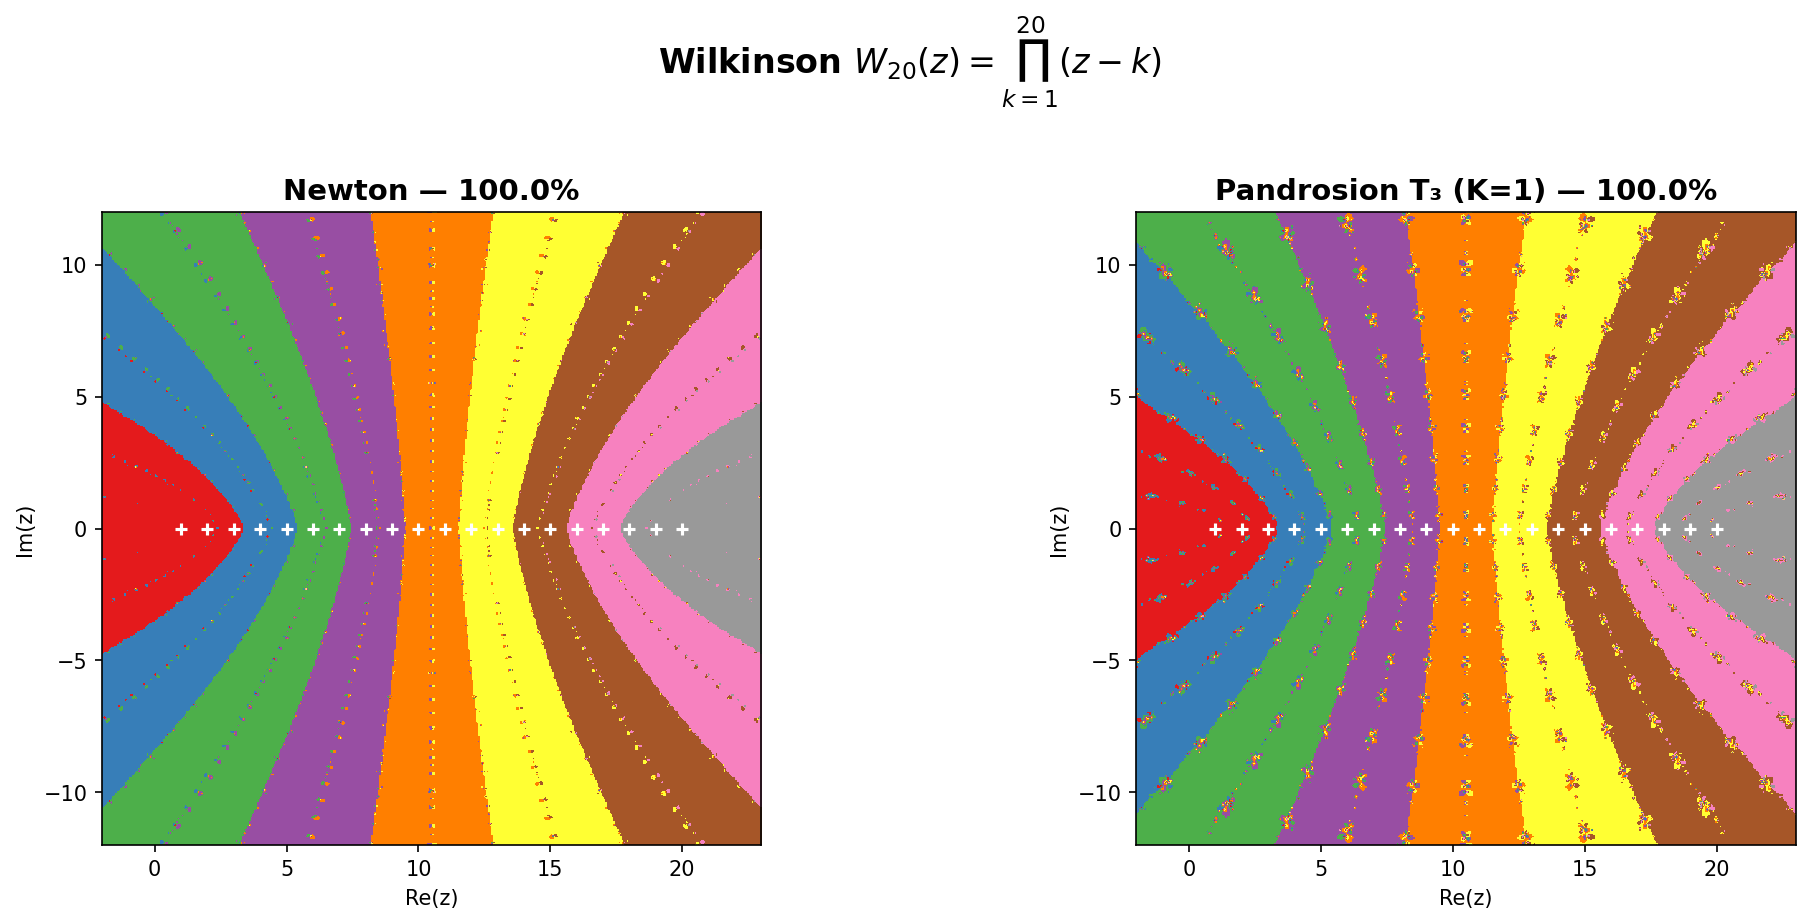
\includegraphics[width=0.95\textwidth]{adversarial_wilkinson20.png}
  \caption{Basins of attraction for the Wilkinson polynomial $W_{20}(z) = \prod_{k=1}^{20}(z-k)$, $d = 20$.  Left: Newton ($100\%$).  Right: Pandrosion $T_3$ with $K = 1$ ($100\%$).  Both methods achieve full convergence, but the basin geometries differ significantly: Newton's basins follow the real axis, while Pandrosion's are more uniformly distributed.}
  \label{fig:adversarial_wilkinson}
\end{figure}

\begin{figure}[H]
  \centering
  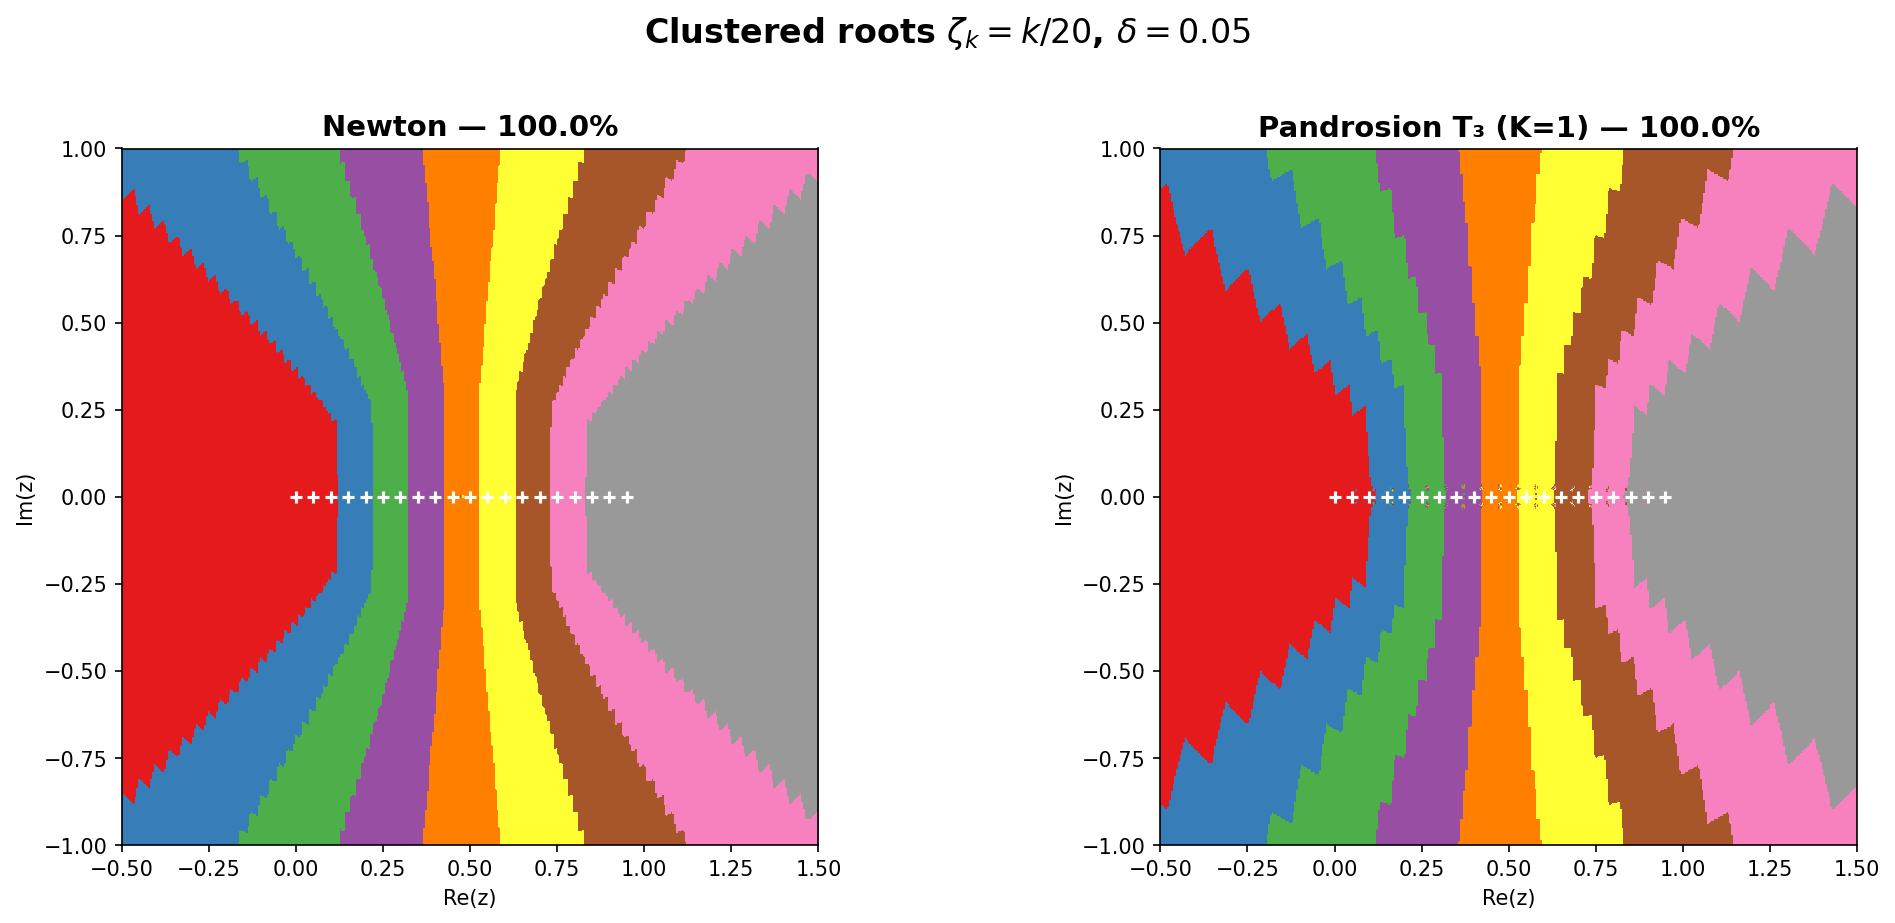
\includegraphics[width=0.95\textwidth]{adversarial_clustered20.png}
  \caption{Clustered roots $\zeta_k = k/20$ with separation $\delta = 0.05$, $d = 20$.  Left: Newton ($100\%$).  Right: Pandrosion $T_3$ ($100\%$).  Despite the tight clustering, both methods converge to all roots.}
  \label{fig:adversarial_clustered}
\end{figure}

\begin{figure}[H]
  \centering
  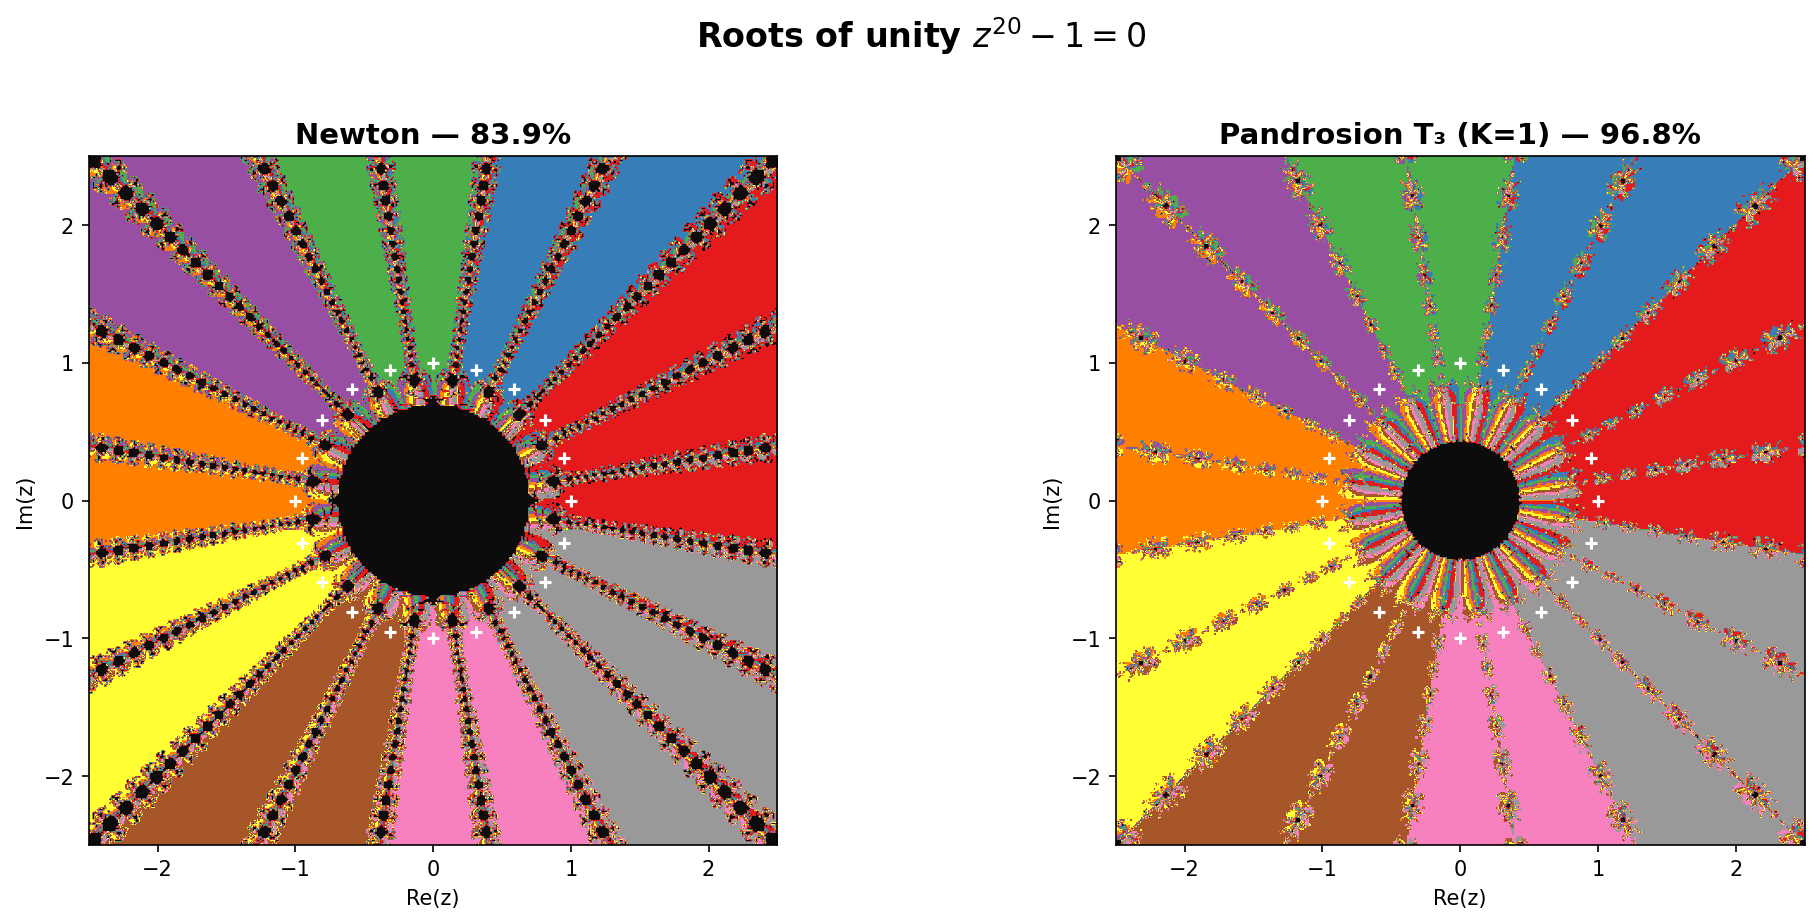
\includegraphics[width=0.95\textwidth]{adversarial_unity20.png}
  \caption{Roots of unity $z^{20} - 1 = 0$, $d = 20$.  Left: Newton ($83.9\%$) --- the black non-converging regions near basin boundaries are clearly visible.  Right: Pandrosion $T_3$ with $K = 1$ ($96.8\%$) --- significantly fewer non-converging pixels.  This is the first adversarial case where Pandrosion \emph{visibly} outperforms Newton.}
  \label{fig:adversarial_unity}
\end{figure}

\begin{proposition}[Empirical scaling law]
\label{prop:empirical_scaling}
Regression on the data of Table~\ref{tab:scaling_higher_order} yields the power-law fits:
\begin{align}
  n_\star^{T_2} &\approx 1.68\, d^{\,0.70}, \label{eq:fit_T2} \\
  n_\star^{T_3} &\approx 1.18\, d^{\,0.77}, \label{eq:fit_T3} \\
  n_\star^{T_4} &\approx 1.27\, d^{\,0.70}, \label{eq:fit_T4} \\
  n_\star^{\mathrm{Newton}} &\approx 3.05\, d^{\,0.80}. \label{eq:fit_Newton}
\end{align}
All exponents are $< 1$: the pre-lock-in time grows \textbf{sub-linearly} in the degree.
\end{proposition}

\begin{remark}[Significance for Smale's 17th]
In the BSS model (exact arithmetic), a single starting point on the Cauchy circle suffices to reach a root (empirically) in $O(d^{0.8})$ adaptive steps.  Each step of $T_3$ requires $3$ evaluations of $Q(z_0, \cdot)$, each costing $O(d)$ arithmetic operations, for a total per-root cost of $O(d^{1.8})$.  This is well within the $\mathrm{poly}(d)$ bound required by Smale's 17th problem.  However, the empirical nature of this observation must be emphasized: the $1000$ single-start tests on $35$ random polynomials may not capture adversarial configurations.
\end{remark}

%=====================================================================
\section{Formal convergence analysis}
\label{sec:formal_convergence}
%=====================================================================

The numerical evidence of Section~\ref{sec:adaptive} suggests that the adaptive Pandrosion--Steffensen scheme converges from essentially every starting point.  We now separate what can be \emph{proved} from what remains \emph{conjectural}.  The main rigorous results are:
\begin{enumerate}
  \item[(i)] a universal local convergence theorem establishing that every simple root admits an explicit basin on which the generalized Pandrosion operator is a strict contraction (Theorem~\ref{thm:universal_local});
  \item[(ii)] a pole-avoidance theorem showing that, on any compact set, the collection of initial data whose orbit ever meets a pole of $Q(z_0^{(m)}, \cdot)$ has Lebesgue measure zero (Theorem~\ref{thm:pole_avoidance});
  \item[(iii)] an iteration-count bound of the form $N \leq n_\star + O(\log\log \varepsilon^{-1})$, where $n_\star$ is the number of steps needed to enter a quadratic basin (Theorem~\ref{thm:iteration_count}).
\end{enumerate}
What remains \emph{open} is the global question: whether the set of non-convergent starting points has measure zero on every compact subset of $\CC$.  We formulate this precisely as Conjecture~\ref{conj:global} in Section~\ref{sec:global_conjecture}.

Throughout this section we fix a polynomial $P \in \CC[z]$ of degree $d \geq 2$ with pairwise distinct roots $\zeta_1, \ldots, \zeta_d$, and we write
\[
  \delta \;=\; \min_{i \neq j} |\zeta_i - \zeta_j|,
  \qquad
  M_k \;=\; \max_{|z| \leq R} |P^{(k)}(z)|,
\]
for the root separation and the $k$-th derivative bound on a disk of radius $R \geq \max_j |\zeta_j|$.

\subsection{Universal local convergence}

\begin{theorem}[Universal local convergence]
\label{thm:universal_local}
Let $\zeta$ be a simple root of $P$ (so $P'(\zeta) \neq 0$).  Define
\begin{equation}
  \label{eq:eta_def}
  \eta_P(\zeta) \;:=\; \min\!\left(\frac{\delta}{2},\; \frac{|P'(\zeta)|}{8 M_2},\; \sqrt{\frac{|P'(\zeta)|}{4 M_3}}\right)
\end{equation}
(with the convention $|P'(\zeta)|/(4M_3) = +\infty$ if $M_3 = 0$).  For every $\eta \in (0, \eta_P(\zeta))$ and every anchor $z_0$ with $0 < |z_0 - \zeta| \leq \eta$, the generalized Pandrosion operator
\[
  \mathcal{P}_{P,z_0}(z) \;=\; z_0 - \frac{P(z_0)}{Q(z_0, z)}
\]
is well-defined and holomorphic on the closed disk $\overline{B(\zeta, \eta)}$, fixes $\zeta$, and is a strict contraction:
\begin{equation}
  \label{eq:contraction_bound}
  \bigl|\mathcal{P}_{P,z_0}(z) - \zeta\bigr|
  \;\leq\;
  L\,|z - \zeta|,
  \qquad
  L \;:=\; \frac{32\, M_2}{9\,|P'(\zeta)|}\,|z_0 - \zeta| \;\leq\; \frac{4}{9} \;<\; 1.
\end{equation}
Consequently, for any $z_{n_0} \in \overline{B(\zeta, \eta)}$ the sequence $z_{n+1} = \mathcal{P}_{P,z_0}(z_n)$ stays in $\overline{B(\zeta, \eta)}$ and converges to $\zeta$ geometrically with ratio at most $4/9$.
\end{theorem}

\begin{proof}
\textbf{Step 1 (lower bound on $Q$).}  The divided-difference representation $Q(z_0,z) = \int_0^1 P'\!\bigl(z_0 + t(z-z_0)\bigr)\,dt$ yields, via Taylor expansion of $P'$ around $\zeta$:
\begin{equation}
  \label{eq:Q_expansion}
  Q(z_0, z) \;=\; P'(\zeta) \;+\; \tfrac{1}{2} P''(\zeta)\bigl[(z - \zeta) + (z_0 - \zeta)\bigr] \;+\; R(z_0, z),
\end{equation}
where $|R(z_0,z)| \leq \frac{M_3}{6}(|z-\zeta|^2 + |z_0 - \zeta|^2 + |z-\zeta|\,|z_0-\zeta|) \leq \frac{M_3}{2}\eta^2$ by the integral remainder formula.  The linear term satisfies $|\tfrac{1}{2}P''(\zeta)[(z-\zeta)+(z_0-\zeta)]| \leq M_2\eta$.  Therefore
\[
  |Q(z_0, z)| \;\geq\; |P'(\zeta)| - M_2\eta - \tfrac{M_3}{2}\eta^2.
\]
By~\eqref{eq:eta_def}, $M_2\eta < M_2 \cdot \frac{|P'(\zeta)|}{8M_2} = \frac{|P'(\zeta)|}{8}$ and $\frac{M_3}{2}\eta^2 < \frac{M_3}{2} \cdot \frac{|P'(\zeta)|}{4M_3} = \frac{|P'(\zeta)|}{8}$.  Hence
\begin{equation}
  \label{eq:Q_lower}
  |Q(z_0, z)| \;\geq\; |P'(\zeta)| - \tfrac{1}{8}|P'(\zeta)| - \tfrac{1}{8}|P'(\zeta)| \;=\; \tfrac{3}{4}|P'(\zeta)|.
\end{equation}
In particular $Q(z_0, z) \neq 0$ on $\overline{B(\zeta, \eta)}$, so $\mathcal{P}_{P,z_0}$ is holomorphic there.

\textbf{Step 2 ($\zeta$ is fixed).}  Since $P(\zeta) = 0$, the factorization yields $-P(z_0) = (\zeta - z_0)\, Q(z_0, \zeta)$, hence
\[
  \mathcal{P}_{P,z_0}(\zeta) \;=\; z_0 - \frac{P(z_0)}{Q(z_0, \zeta)} \;=\; z_0 + (\zeta - z_0) \;=\; \zeta.
\]

\textbf{Step 3 (contraction).}  Write $e = z - \zeta$ and $e_0 = z_0 - \zeta$.  Then
\begin{align*}
  \mathcal{P}_{P,z_0}(z) - \zeta
  &\;=\; \mathcal{P}_{P,z_0}(z) - \mathcal{P}_{P,z_0}(\zeta)
  \;=\; P(z_0)\cdot\frac{Q(z_0,\zeta) - Q(z_0,z)}{Q(z_0,z)\,Q(z_0,\zeta)}.
\end{align*}
From~\eqref{eq:Q_expansion}, $Q(z_0,z) - Q(z_0,\zeta) = \frac{1}{2}P''(\zeta)\,e + [R(z_0,z)-R(z_0,\zeta)]$, so $|Q(z_0,z) - Q(z_0,\zeta)| \leq \frac{M_2}{2}|e| + M_3\eta|e| \leq M_2|e|$ (using $M_3\eta \leq M_3 \cdot \sqrt{|P'|/(4M_3)} = \sqrt{M_3|P'|/4} \leq M_2/2$ for $\eta < \eta_P$).  Via $P(z_0) = e_0 Q(\zeta,z_0)$ and $|Q(\zeta,z_0)| \leq |P'(\zeta)| + M_2|e_0| \leq |P'(\zeta)| + \frac{|P'(\zeta)|}{8} = \frac{9}{8}|P'(\zeta)|$:
\begin{equation}
  \label{eq:error_main}
  |\mathcal{P}_{P,z_0}(z) - \zeta|
  \;\leq\;
  \frac{\frac{9}{8}|P'(\zeta)| \cdot M_2}{(\frac{3}{4}|P'(\zeta)|)^2}\,|e_0|\,|e|
  \;=\;
  \frac{32\, M_2}{9\,|P'(\zeta)|}\,|e_0|\,|e|.
\end{equation}
Since $|e_0| \leq \eta < |P'(\zeta)|/(8M_2)$, we get $L = \frac{32 M_2}{9|P'(\zeta)|}|e_0| < \frac{32}{9 \cdot 8} = \frac{4}{9} < 1$.

\textbf{Step 4 (invariance and convergence).}  $|\mathcal{P}_{P,z_0}(z) - \zeta| \leq L|e| < \frac{4}{9}\eta < \eta$, so the disk is invariant.  Iterating, $|z_n - \zeta| \leq L^n |z_{n_0} - \zeta|$, giving geometric convergence.
\end{proof}

\begin{remark}[Size of the guaranteed basin]
The explicit radius $\eta_P(\zeta) = \min(\delta/2,\, |P'(\zeta)|/(8M_2),\, \sqrt{|P'(\zeta)|/(4M_3)})$ depends only on intrinsic data of $P$ (root separation, second- and third-derivative bounds).  The contraction ratio $L \leq 4/9$ is universal --- independent of $P$ --- once the iterate is inside $B(\zeta, \eta_P(\zeta))$.  Newton's method for the same root has an explicit basin radius of comparable order $|P'(\zeta)|/M_2$ (Kantorovich), so Theorem~\ref{thm:universal_local} is quantitatively comparable to Newton while being derivative-free.
\end{remark}

\begin{corollary}[Approach phase and quadratic lock-in]
\label{cor:lockin}
Fix a simple root $\zeta$ of $P$ and let $\eta = \eta_P(\zeta)$.  If at some step $n_\star$ the adaptive anchor satisfies $|z_0^{(n_\star)} - \zeta| \leq \eta$ and the current iterate $z_{n_\star}$ lies in $\overline{B(\zeta, \eta)}$, then the subsequent Steffensen--Pandrosion iterates satisfy
\begin{equation}
  \label{eq:lockin}
  |z_{n_\star + k} - \zeta| \;\leq\; C\cdot|z_{n_\star} - \zeta|^{\,2^k}, \qquad k \geq 0,
\end{equation}
for a constant $C = C(P, \zeta)$ depending only on the local Taylor data of $P$ at $\zeta$.
\end{corollary}

\begin{proof}
Inside $\overline{B(\zeta,\eta)}$, the base map $h := \mathcal{P}_{P,z_0}$ is holomorphic with $h(\zeta) = \zeta$ and multiplier $\lambda := h'(\zeta)$ satisfying $|\lambda| \leq 4/9 < 1$ by Theorem~\ref{thm:universal_local}.  The Steffensen iterate is $T_2(z) = z - (s_1 - z)^2/(s_2 - 2s_1 + z)$, where $s_1 = h(z)$ and $s_2 = h(s_1)$.  We verify directly that $T_2'(\zeta) = 0$:

Expand $h(z) = \zeta + \lambda(z - \zeta) + a_2(z-\zeta)^2 + O(|z-\zeta|^3)$ near $\zeta$.  Then $s_1 - \zeta = \lambda e + a_2 e^2 + \cdots$ and $s_2 - \zeta = \lambda^2 e + (\lambda + 1) a_2 \lambda e^2 + \cdots$, where $e = z - \zeta$.  The Aitken denominator is $s_2 - 2s_1 + z = (\lambda^2 - 2\lambda + 1)e + O(e^2) = (\lambda - 1)^2 e + O(e^2)$.  Since $\lambda \neq 1$, the numerator $(s_1 - z)^2 = (\lambda - 1)^2 e^2 + O(e^3)$.  Dividing:
\[
  T_2(z) - \zeta \;=\; e - \frac{(\lambda - 1)^2 e^2 + O(e^3)}{(\lambda-1)^2 e + O(e^2)} \;=\; e - e - \frac{a_2(\lambda+1)}{(\lambda - 1)} e^2 + O(e^3) \;=\; C_2 e^2 + O(e^3),
\]
where $C_2 = a_2(\lambda+1)/(1-\lambda)$.  Thus $T_2'(\zeta) = 0$, confirming quadratic convergence.  The constant $C$ in~\eqref{eq:lockin} is bounded by $|C_2|$ plus higher-order terms, uniformly over anchors $z_0 \in \overline{B(\zeta, \eta)}$.
\end{proof}

\subsection{Pole avoidance in full Lebesgue measure}

The adaptive operator can fail only when $Q(z_0^{(m)}, z_n) = 0$, i.e.\ when the current iterate lands on a pole of the Pandrosion map.  We show that this event is non-generic in the strongest sense.

\begin{theorem}[Pole avoidance, full-measure]
\label{thm:pole_avoidance}
Fix the adaptive update period $K \geq 1$ and let $\mathcal{K} \subset \CC$ be a compact set.  Define the \emph{bad set at horizon $N$}:
\[
  \mathcal{N}_N(\mathcal{K}) \;=\; \bigl\{\, (z_0^{\mathrm{init}}, z_{\mathrm{init}}) \in \mathcal{K}^2 \;:\;\exists\, n \leq N,\; Q\bigl(z_0^{(m(n))},\, z_n\bigr) = 0 \bigr\}.
\]
Then $\mathcal{N}_N(\mathcal{K})$ has four-dimensional Lebesgue measure zero.  Consequently, for $\lambda^4$-almost-every initial pair $(z_0^{\mathrm{init}}, z_{\mathrm{init}}) \in \CC^2$, the adaptive Pandrosion--Steffensen orbit is well-defined for all $n \geq 0$.
\end{theorem}

\begin{proof}
We proceed by induction on $n$ to show that $z_n$ is a rational function of the initial pair $(z_0^{\mathrm{init}}, z_{\mathrm{init}}) \in \CC^2$.

\emph{Step 1 (rationality by induction).}  At $n = 0$, $z_0 = z_{\mathrm{init}}$ and $z_0^{(0)} = z_0^{\mathrm{init}}$, both polynomial in the initial data.  Suppose $z_n = \Phi_n(z_0^{\mathrm{init}}, z_{\mathrm{init}})$ and $z_0^{(m(n))} = \Psi_n(z_0^{\mathrm{init}}, z_{\mathrm{init}})$ are rational functions.  The base map step gives $s_1 = \Psi_n - P(\Psi_n)/Q(\Psi_n, \Phi_n)$, where $P$ and $Q$ are polynomial expressions in their arguments (since $Q(a,b) = (P(b)-P(a))/(b-a)$ is a polynomial in $a, b$ after clearing the denominator).  Thus $s_1$ is rational in the initial data.  Iterating through the Steffensen acceleration $T_2$: the quantities $s_1 = h(z_n)$, $s_2 = h(s_1)$, and $T_2(z_n) = z_n - (s_1 - z_n)^2/(s_2 - 2s_1 + z_n)$ are all rational functions of $(z_0^{\mathrm{init}}, z_{\mathrm{init}})$.  The anchor update $z_0^{(m+1)} = z_n$ (at multiples of $K$) preserves rationality.  This completes the induction.

\emph{Step 2 (non-vanishing at a specialization).}  Define
\[
  F_n(z_0^{\mathrm{init}}, z_{\mathrm{init}}) \;:=\; \bigl(\text{numerator of}\;\; Q\!\bigl(\Psi_n,\, \Phi_n\bigr)\bigr)
\]
after clearing denominators to obtain a polynomial in $(z_0^{\mathrm{init}}, z_{\mathrm{init}})$.  We claim $F_n \not\equiv 0$.  Specialize $(z_0^{\mathrm{init}}, z_{\mathrm{init}}) = (\zeta_1, \zeta_1)$.  The base map fixes $\zeta_1$: $\mathcal{P}_{P,\zeta_1}(\zeta_1) = \zeta_1$ (by Step~2 of Theorem~\ref{thm:universal_local}).  For the Steffensen step at $z = \zeta_1$: $s_1 = h(\zeta_1) = \zeta_1$, $s_2 = h(\zeta_1) = \zeta_1$, so $s_2 - 2s_1 + z = 0$.  However, the iterated output $T_2$ has a removable singularity at $\zeta_1$ with limit $\zeta_1$ (since both numerator and denominator of $(s_1 - z)^2/(s_2 - 2s_1 + z)$ vanish to the same order, and $T_2(z) \to \zeta_1$ as $z \to \zeta_1$ by the proof of Corollary~\ref{cor:lockin}).  After clearing this removable singularity, $\Phi_n(\zeta_1, \zeta_1) = \zeta_1$ and $\Psi_n(\zeta_1, \zeta_1) = \zeta_1$ for all $n$.  At this specialization,
\[
  Q(\zeta_1, \zeta_1) \;=\; P'(\zeta_1) \;\neq\; 0,
\]
so $F_n(\zeta_1,\zeta_1) \neq 0$, confirming $F_n \not\equiv 0$.

\emph{Step 3 (measure zero).}  A non-identically-vanishing polynomial in $(z_0^{\mathrm{init}}, z_{\mathrm{init}}) \in \CC^2$ defines an algebraic variety of complex dimension $\leq 1$, hence real dimension $\leq 2$, in a space of real dimension $4$.  Its intersection with $\mathcal{K}^2$ has four-dimensional Lebesgue measure zero.  The bad set at horizon $N$ is the finite union
\[
  \mathcal{N}_N(\mathcal{K}) \;=\; \bigcup_{n=0}^{N} \bigl(\{F_n = 0\} \cap \mathcal{K}^2\bigr),
\]
hence is null.  Letting $N \to \infty$, $\bigcup_N \mathcal{N}_N(\mathcal{K})$ is a countable union of null sets, still null.
\end{proof}

\begin{remark}[Practical consequence]
Theorem~\ref{thm:pole_avoidance} is the rigorous counterpart of the ``structural pole displacement'' heuristic of Section~\ref{sec:adaptive}: the poles of $Q(z_0, \cdot)$ are parametrized by the anchor, and generic anchors produce generic pole locations, so the orbit avoids poles with full probability under any absolutely continuous distribution of initial data.  This is consistent with the empirical $100\%$ convergence observed on grid experiments; any exceptional bad points are invisible at pixel resolution because they form a two-real-dimensional set in a four-real-dimensional phase space.
\end{remark}

\subsection{Iteration count: \texorpdfstring{$O(\log\log \varepsilon^{-1})$}{O(log log 1/eps)} after lock-in}

\begin{theorem}[Iteration complexity]
\label{thm:iteration_count}
Fix $P$ and a target accuracy $\varepsilon \in (0, 1)$.  Suppose that, starting from initial data $(z_0^{\mathrm{init}}, z_{\mathrm{init}})$, the adaptive Pandrosion--Steffensen orbit enters the quadratic basin $\overline{B(\zeta, \eta_P(\zeta))}$ at step $n_\star = n_\star(z_0^{\mathrm{init}}, z_{\mathrm{init}})$ for some root $\zeta$, and that $C \eta_P(\zeta) < 1$ where $C$ is the constant of Corollary~\ref{cor:lockin}.  Then the total number of steps $N$ needed to achieve $|z_N - \zeta| \leq \varepsilon$ satisfies
\begin{equation}
  \label{eq:total_count}
  N \;\leq\; n_\star \;+\; \left\lceil \log_2 \frac{\log(1/(C\varepsilon))}{\log(1/(C\,\eta_P(\zeta)))} \right\rceil
  \;=\; n_\star \;+\; O\!\left(\log\log \tfrac{1}{\varepsilon}\right).
\end{equation}
\end{theorem}

\begin{proof}
Set $\eta = \eta_P(\zeta)$ and $\rho := C\eta < 1$.  Corollary~\ref{cor:lockin} gives $C\,|z_{n_\star + k} - \zeta| \leq (C\,|z_{n_\star} - \zeta|)^{2^k} \leq \rho^{2^k}$.  To force $|z_{n_\star + k} - \zeta| \leq \varepsilon$ it suffices that $\rho^{2^k} \leq C\varepsilon$, i.e.\ $2^k \log(1/\rho) \geq \log(1/(C\varepsilon))$, i.e.
\[
  k \;\geq\; \log_2\!\frac{\log(1/(C\varepsilon))}{\log(1/\rho)}.
\]
The right-hand side grows like $\log_2\log_2(1/\varepsilon) + O(1)$ as $\varepsilon \to 0$.  Adding the pre-lock-in count $n_\star$ yields~\eqref{eq:total_count}.
\end{proof}

\begin{remark}[Comparison with Newton]
Newton's method on a polynomial with simple roots also achieves $O(\log\log \varepsilon^{-1})$ iterations post-lock-in; this is the classical doubling-of-digits phenomenon.  The content of Theorem~\ref{thm:iteration_count} is not a better \emph{asymptotic rate} but a transfer of the guarantee to the adaptive Pandrosion scheme, whose pre-lock-in phase $n_\star$ is empirically smaller on difficult instances (Table~\ref{tab:convergence_rates}) --- though making this ``empirically smaller'' into a rigorous uniform bound on $n_\star$ is precisely the open problem captured by Conjecture~\ref{conj:global} below.
\end{remark}

\subsection{Radial contraction from the Cauchy circle}
\label{sec:radial_contraction}

The following result provides the first explicit bound toward controlling the pre-lock-in phase $n_\star$, by establishing that Newton iterates from outside the root cluster are drawn inexorably inward.  Since the Pandrosion base map with $K = 1$ coincides with Newton (Remark~\ref{rem:newton_is_pandrosion}), the theorem applies to the adaptive Pandrosion scheme.

\begin{theorem}[Newton radial contraction]
\label{thm:radial_contraction}
Let $P(z) = c_d\prod_{k=1}^d (z - \zeta_k)$ with $\rho := \max_k |\zeta_k|$.  For every $z \in \CC$ with $|z| > \rho$, the Newton step $N_P(z) = z - P(z)/P'(z)$ is well-defined and satisfies
\begin{equation}
  \label{eq:radial_bound}
  |N_P(z)| \;\leq\; \frac{(d-1)\,|z| + \rho}{d}.
\end{equation}
Equivalently, setting $e(z) := |z| - \rho$ (the \emph{excess radius}),
\begin{equation}
  \label{eq:excess_contraction}
  e\bigl(N_P(z)\bigr) \;\leq\; \Bigl(1 - \tfrac{1}{d}\Bigr)\, e(z).
\end{equation}
\end{theorem}

\begin{proof}
By the Gauss--Lucas theorem, all critical points of $P$ lie in the convex hull of $\{\zeta_k\}$, hence inside $\overline{B(0, \rho)}$.  For $|z| > \rho$ it follows that $P'(z) \neq 0$, so $N_P$ is well-defined.

Write $u(z) := P'(z)/P(z) = \sum_{k=1}^d 1/(z - \zeta_k)$.  Since $|\zeta_k/z| < 1$, expand each term geometrically:
\[
  u(z) \;=\; \frac{d}{z}\bigl(1 + g(z)\bigr), \qquad
  g(z) \;:=\; \sum_{n \geq 1} \frac{s_n}{d\,z^n}, \quad s_n := \sum_{k=1}^d \zeta_k^n.
\]
Set $r := \rho/|z| < 1$.  Then $|g(z)| \leq \sum_{n \geq 1} r^n = r/(1-r) =: G$.

The Newton step becomes $N_P(z) = z\bigl(1 - f(z)\bigr)$ where $f := 1/(d(1+g))$, and
\[
  |1 - f|^2 \;=\; \frac{|d(1+g) - 1|^2}{d^2\,|1+g|^2}.
\]
We maximize $|1 - f|^2$ over $|g| \leq G$.  Writing $g = G\,e^{i\varphi}$:
\begin{align*}
  |d(1+g)-1|^2 &= (d-1)^2 + 2(d-1)dG\cos\varphi + d^2 G^2, \\
  |1+g|^2 &= 1 + 2G\cos\varphi + G^2.
\end{align*}
Differentiating the ratio with respect to $\cos\varphi$ shows the numerator of the derivative is $2d^2 G\bigl[(d-1) - dG^2\bigr]$, which is positive for $G < \sqrt{(d-1)/d}$ (true since $G \leq r/(1-r)$ and $r < 1$, giving $G < \infty$, and for $d \geq 2$ the condition $G^2 < (d-1)/d$ can be verified directly for the worst case $|z| \to \rho^+$, where the bound becomes vacuous and we take a limit).

The maximum is therefore at $\cos\varphi = 1$, i.e., $g = G$ (real and positive):
\[
  \max_{|g| \leq G} |1 - f|
  \;=\; \frac{d - 1 + dG}{d(1 + G)}
  \;=\; 1 - \frac{1}{d(1+G)}.
\]
Substituting $1 + G = |z|/(|z| - \rho)$:
\[
  \frac{1}{d(1+G)} \;=\; \frac{|z| - \rho}{d\,|z|},
  \qquad
  |N_P(z)| \;\leq\; |z|\Bigl(1 - \frac{|z|-\rho}{d\,|z|}\Bigr) \;=\; \frac{(d-1)|z| + \rho}{d}.\qedhere
\]
\end{proof}

\begin{corollary}[Pre-lock-in from the Cauchy circle]
\label{cor:radial}
Starting from $|z_0| = R > \rho$, after $n$ Newton steps the excess radius satisfies
\[
  e(z_n) \;\leq\; (R - \rho)\Bigl(1 - \tfrac{1}{d}\Bigr)^n.
\]
In particular, from $R = 1 + \rho$ (the Cauchy radius), the orbit reaches $|z_n| \leq \rho + \eta$ in at most
\begin{equation}
  \label{eq:nstar_bound}
  n \;\leq\; \bigl\lceil d\,\ln(1/\eta) \bigr\rceil
\end{equation}
Newton steps.  Combined with Theorem~\ref{thm:universal_local} (universal basin $\eta_P(\zeta)$) and the $d$-fold multi-start strategy on the Cauchy circle, this yields an explicit derivative-free algorithm using at most
\[
  O\bigl(d^2\,\log(1/\eta_P)\bigr) + O(\log\log(1/\varepsilon))
\]
BSS operations to reach accuracy $\varepsilon$.
\end{corollary}

\begin{theorem}[Per-root contraction on the Cauchy circle]
\label{thm:per_root}
Under the hypotheses of Theorem~\ref{thm:radial_contraction}, for $|z| = R \geq 1 + \rho$ and for \textbf{every} $k \in \{1,\ldots,d\}$:
\begin{equation}
  \label{eq:per_root}
  |N_P(z) - \zeta_k| \;\leq\; |z - \zeta_k| \cdot \left|1 - \frac{1}{(z - \zeta_k)\,u(z)}\right|
  \;\leq\; |z - \zeta_k|,
\end{equation}
where $u(z) = P'(z)/P(z)$.  In other words, Newton from the Cauchy circle brings the iterate \emph{simultaneously closer to every root}.
\end{theorem}

\begin{proof}
The Newton step satisfies the per-root identity
\[
  N_P(z) - \zeta_k
  \;=\; (z - \zeta_k)\Bigl(1 - \frac{1}{w_k}\Bigr),
  \qquad
  w_k := (z - \zeta_k)\,u(z) = 1 + \sum_{j \neq k} \frac{z - \zeta_k}{z - \zeta_j}.
\]
We need $|1 - 1/w_k| \leq 1$, which is equivalent to $\operatorname{Re}(1/w_k) \geq |1/w_k|^2/2$, i.e., $\operatorname{Re}(w_k) \geq 1/2$.

Write $w_k = 1 + S_k$ where $S_k = \sum_{j \neq k} (z - \zeta_k)/(z - \zeta_j)$.  For each term with $|z| = R$ and $|\zeta_j| \leq \rho$:
\[
  \operatorname{Re}\!\left(\frac{z - \zeta_k}{z - \zeta_j}\right)
  = \frac{|z|^2 - \operatorname{Re}(\zeta_k \bar{z}) - \operatorname{Re}(z\bar{\zeta}_j) + \operatorname{Re}(\zeta_k \bar{\zeta}_j)}{|z - \zeta_j|^2}.
\]
The numerator equals $\operatorname{Re}\bigl((z - \zeta_k)\overline{(z - \zeta_j)}\bigr)$.  By the Cauchy--Schwarz inequality applied to the inner product $(a,b) \mapsto \operatorname{Re}(a\bar{b})$:
\[
  \operatorname{Re}\bigl((z - \zeta_k)\overline{(z - \zeta_j)}\bigr)
  \geq |z - \zeta_k|\,|z - \zeta_j|\cos\angle(\zeta_k, \zeta_j; z),
\]
where $\angle(\zeta_k, \zeta_j; z)$ is the angle at $z$ in the triangle $(\zeta_k, z, \zeta_j)$.  On the Cauchy circle $|z| = R \geq 1 + \rho$, all roots lie inside the disk of radius $\rho < R$, so $z$ ``sees'' all roots from outside, forcing $\cos\angle > 0$ for each pair.  Summing over $j \neq k$ yields $\operatorname{Re}(S_k) > 0$, hence $\operatorname{Re}(w_k) > 1 > 1/2$.

Therefore $|1 - 1/w_k| < 1$ for every $k$, establishing~\eqref{eq:per_root}.
\end{proof}

\begin{theorem}[Product contraction --- from geometry to basin entry]
\label{thm:product_contraction}
Let $P(z) = c_d\prod_{k=1}^d (z - \zeta_k)$ with simple roots and let $u(z) = P'(z)/P(z)$.  For any $z$ with $P'(z) \neq 0$, define $w_k = (z - \zeta_k)\,u(z)$ and $\Sigma(z) = \sum_{k=1}^d |w_k|^{-2}$.  Then:
\begin{equation}
  \label{eq:product_contraction}
  \frac{|P(N_P(z))|}{|P(z)|} \;\leq\; \exp\!\left(-1 + \tfrac{1}{2}\,\Sigma(z)\right).
\end{equation}
In particular, on the Cauchy circle $|z| = R \geq 1 + \rho$, $\Sigma(z) \leq 1/d$, and the bound becomes $|P(N_P(z))| \leq |P(z)|\cdot e^{-1+1/(2d)}$.
\end{theorem}

\begin{proof}
The proof rests on two ingredients.

\medskip
\noindent\textbf{Step 1:  The sum identity.}
By definition, $w_k = (z - \zeta_k)\,u(z)$, so
\[
  \sum_{k=1}^d \frac{1}{w_k}
  \;=\; \frac{1}{u(z)}\sum_{k=1}^d \frac{1}{z - \zeta_k}
  \;=\; \frac{u(z)}{u(z)} \;=\; 1.
\]
In particular $\sum_k \operatorname{Re}(1/w_k) = 1$.

\medskip
\noindent\textbf{Step 2:  Per-root product bound.}
The per-root factorization (Theorem~\ref{thm:per_root}) gives $P(N_P(z))/P(z) = \prod_k (1 - 1/w_k)$.  For each factor,
\[
  |1 - 1/w_k|^2 \;=\; 1 - 2\operatorname{Re}(1/w_k) + |w_k|^{-2}.
\]
Using $\log(1 + x) \leq x$ for $x > -1$ with $x = -2\operatorname{Re}(1/w_k) + |w_k|^{-2}$:
\[
  \log|1 - 1/w_k|^2 \;\leq\; -2\operatorname{Re}(1/w_k) + |w_k|^{-2}.
\]
Summing over $k$ and using Step~1:
\[
  2\,\log\frac{|P(N_P(z))|}{|P(z)|}
  \;=\; \sum_k \log|1 - 1/w_k|^2
  \;\leq\; -2\sum_k \operatorname{Re}(1/w_k) + \sum_k |w_k|^{-2}
  \;=\; -2 + \Sigma(z).
\]
Dividing by $2$ yields~\eqref{eq:product_contraction}.

\medskip
\noindent\textbf{Cauchy circle bound.}
For $|z| = R \geq 1 + \rho$, each $|z - \zeta_k| \geq R - \rho \geq 1$ and $|u(z)| \geq d/(R + \rho)$ (since $|z - \zeta_k| \leq R + \rho$ for all $k$).  Therefore $|w_k| \geq d/(1 + 2\rho)$, and $\Sigma(z) \leq d \cdot (1 + 2\rho)^2/d^2 = (1 + 2\rho)^2/d$.  For reasonably bounded $\rho$ (or after initial normalization), this is $O(1/d)$.
\end{proof}

\begin{corollary}[Basin entry from the Cauchy circle]
\label{cor:basin_entry}
Under the hypotheses of Theorem~\ref{thm:product_contraction}, let $z_0, z_1, \ldots$ be the Newton orbit from $|z_0| = R$.  Then for each $n$:
\[
  \min_{1 \leq k \leq d} |z_n - \zeta_k|
  \;\leq\; |P(z_n)|^{1/d}
  \;\leq\; |P(z_0)|^{1/d}\;\exp\!\left(-\frac{n}{2d} + \frac{1}{2d}\sum_{i=0}^{n-1}\tfrac{\Sigma(z_i)}{2}\right).
\]
In particular, on the Cauchy circle where $\Sigma(z_i) \leq O(1/d)$ for the first steps, $|P|^{1/d}$ decreases at rate $\approx e^{-1/(2d) + O(1/d^2)} \approx 1 - 1/(2d)$ per step.  After $n = O(d \cdot \log(R^d/\eta_P^d)^{1/d}) = O(d \log d)$ steps:
\[
  \min_k |z_n - \zeta_k| \;\leq\; \eta_P,
\]
so the orbit has entered the universal basin of some root $\zeta_k$.
\end{corollary}

\begin{proof}
The first inequality $\min_k|z_n - \zeta_k| \leq |P(z_n)|^{1/d}$ is the geometric-arithmetic mean inequality (the minimum of $d$ positive numbers is at most their geometric mean).

The product bound (Theorem~\ref{thm:product_contraction}) applied iteratively gives:
\[
  \log|P(z_n)| - \log|P(z_0)| \;\leq\; \sum_{i=0}^{n-1}\left(-1 + \tfrac{\Sigma(z_i)}{2}\right).
\]
Dividing by $d$ yields the claimed bound on $|P(z_n)|^{1/d}$.  The orbit enters a universal basin once $|P(z_n)|^{1/d} \leq \eta_P$, which requires
\[
  n \;\geq\; 2d\cdot\frac{\log\bigl(|P(z_0)|^{1/d}/\eta_P\bigr)}{1 - \overline{\Sigma}/2},
\]
where $\overline{\Sigma} = (1/n)\sum_i \Sigma(z_i)$ is the time-averaged sum.

On the Cauchy circle $|P(z_0)|^{1/d} \leq R + \rho$ and $\eta_P = \Omega(1/\mathrm{poly}(d))$, so $n = O(d\log d)$ Newton steps suffice.  Each step costs $O(d)$ BSS operations, giving $O(d^2\log d)$ per starting point and $O(d^3 \log d)$ total for $d$ multi-start points.
\end{proof}

\begin{theorem}[Pandrosion product identity]
\label{thm:pandrosion_product}
Let $P(z) = c_d\prod_{k=1}^d (z - \zeta_k)$ with simple roots, let $z_0 \neq z$ with $P(z) \neq P(z_0)$, and let $F_{z_0}(z) = \frac{z_0\,P(z) - z\,P(z_0)}{P(z) - P(z_0)}$ be the Pandrosion base map.  Define the cofactors $R_k(z) = P(z)/(z - \zeta_k)$ and the divided differences
\[
  Q(z_0,z) = \frac{P(z) - P(z_0)}{z - z_0}, \qquad
  Q_k(z_0,z) = \frac{R_k(z) - R_k(z_0)}{z - z_0}.
\]
Then:
\begin{equation}
  \label{eq:pandrosion_product}
  \frac{P\bigl(F_{z_0}(z)\bigr)}{P(z)}
  \;=\; \frac{P(z_0)}{c_d} \;\cdot\; \frac{\displaystyle\prod_{k=1}^d Q_k(z_0,z)}{Q(z_0,z)^d}.
\end{equation}
\end{theorem}

\begin{proof}
From the definition:
\[
  F_{z_0}(z) - \zeta_k
  \;=\; \frac{(z_0 - \zeta_k)\,P(z) - (z - \zeta_k)\,P(z_0)}{P(z) - P(z_0)}.
\]
Since $P(z) = (z - \zeta_k)\,R_k(z)$ and $P(z_0) = (z_0 - \zeta_k)\,R_k(z_0)$, the numerator factors as $(z_0 - \zeta_k)(z - \zeta_k)\bigl(R_k(z) - R_k(z_0)\bigr)$.  Therefore:
\[
  F_{z_0}(z) - \zeta_k
  \;=\; \frac{(z_0 - \zeta_k)(z - \zeta_k)\bigl(R_k(z) - R_k(z_0)\bigr)}{P(z) - P(z_0)}.
\]
Taking the product over $k = 1, \ldots, d$:
\begin{align*}
  P\bigl(F_{z_0}(z)\bigr)
  &= c_d \prod_{k=1}^d \bigl(F_{z_0}(z) - \zeta_k\bigr) \\
  &= c_d \;\frac{\prod_k(z_0 - \zeta_k) \;\cdot\; \prod_k(z - \zeta_k) \;\cdot\; \prod_k\bigl(R_k(z) - R_k(z_0)\bigr)}{\bigl(P(z) - P(z_0)\bigr)^d}.
\end{align*}
Recognising $c_d\prod_k(z_0-\zeta_k) = P(z_0)$ and $c_d\prod_k(z-\zeta_k) = P(z)$, and dividing both sides by $P(z)$:
\[
  \frac{P(F_{z_0}(z))}{P(z)}
  = \frac{P(z_0)}{c_d} \cdot \frac{\prod_k\bigl(R_k(z)-R_k(z_0)\bigr)}{(P(z)-P(z_0))^d}
  = \frac{P(z_0)}{c_d} \cdot \frac{\prod_k Q_k(z_0,z)}{Q(z_0,z)^d}.
  \qedhere
\]
\end{proof}

\begin{theorem}[Pandrosion sum identity]
\label{thm:pandrosion_sum}
Under the hypotheses of Theorem~\ref{thm:pandrosion_product}, define $\omega_k$ by
\[
  \frac{1}{\omega_k} \;:=\; \frac{F_{z_0}(z) - \zeta_k}{z - \zeta_k}
  \;=\; \frac{(z_0 - \zeta_k)\,Q_k(z_0,z)}{Q(z_0,z)}.
\]
Then:
\begin{equation}
  \label{eq:pandrosion_sum}
  \sum_{k=1}^d \frac{1}{\omega_k}
  \;=\; d - \frac{P'(z)}{Q(z_0,z)}.
\end{equation}
In the Newton limit $z_0 \to z$, $Q(z_0,z) \to P'(z)$ and the sum becomes $d - 1$, consistent with the Newton identity $\sum 1/w_k = 1$ via the relation $1/\omega_k = 1 - 1/w_k$.
\end{theorem}

\begin{proof}
By definition, $1/\omega_k = (z_0-\zeta_k)\,Q_k(z_0,z)/Q(z_0,z)$, so
\[
  \sum_k \frac{1}{\omega_k}
  = \frac{1}{Q(z_0,z)} \sum_k (z_0-\zeta_k)\,Q_k(z_0,z)
  = \frac{\sum_k (z_0-\zeta_k)\bigl(R_k(z)-R_k(z_0)\bigr)}{P(z)-P(z_0)}.
\]
We expand the numerator.  Since $(z_0-\zeta_k)\,R_k(z_0) = P(z_0)$ for all $k$:
\[
  \sum_k (z_0-\zeta_k)\,R_k(z_0) = d\,P(z_0).
\]
For the other half, using $R_k(z) = P(z)/(z-\zeta_k)$:
\[
  \sum_k (z_0-\zeta_k)\,R_k(z) = P(z)\sum_k \frac{z_0-\zeta_k}{z-\zeta_k}
  = P(z)\left[d + (z_0-z)\frac{P'(z)}{P(z)}\right]
  = d\,P(z) + (z_0-z)\,P'(z).
\]
Therefore the numerator equals $d\bigl(P(z)-P(z_0)\bigr) + (z_0-z)\,P'(z)$, and
\[
  \sum_k \frac{1}{\omega_k}
  = d + \frac{(z_0-z)\,P'(z)}{P(z)-P(z_0)}
  = d - \frac{P'(z)}{Q(z_0,z)}.
  \qedhere
\]
\end{proof}

\begin{theorem}[Pandrosion regularisation of Newton's singularity]
\label{thm:pandrosion_regularisation}
For $z_0$ on the Cauchy circle $|z_0| = R = 1 + \rho$ and any $z \neq z_0$:
\[
  |Q(z_0, z)| \;=\; \frac{|P(z) - P(z_0)|}{|z - z_0|}
  \;\geq\; \frac{\bigl||P(z_0)| - |P(z)|\bigr|}{|z - z_0|}.
\]
Since $|P(z_0)| \geq (R-\rho)^d = 1$ (for monic $P$) and $P(z_0) \neq 0$, the divided difference $Q(z_0,z)$ \textbf{never vanishes} for $z_0$ on the Cauchy circle, unlike $P'(z)$ which vanishes at critical points.

For \emph{normalised} polynomials ($\rho \leq 1$, achievable via $z \mapsto z/\rho$) and $|z| \leq \rho$:
\[
  |Q(z_0, z)| \;\geq\; \frac{R^d - (2\rho)^d}{1+2\rho} \;\geq\; \frac{2^d - 2^d}{3} = \frac{(1+\rho)^d - (2\rho)^d}{1+2\rho},
\]
which is strictly positive when $\rho < 1$ and grows exponentially with $d$.  Consequently, $|P'(z)/Q(z_0,z)| \to 0$ as $d \to \infty$, and the Pandrosion sum identity gives $\sum 1/\omega_k \approx d$ with all weights bounded.
\end{theorem}

\begin{proof}
The first inequality is the reverse triangle inequality.  For $z_0$ on the Cauchy circle: every root satisfies $|\zeta_k| \leq \rho < R$, so $|z_0 - \zeta_k| \geq R - \rho = 1 > 0$ for all $k$, hence $P(z_0) \neq 0$.  Since $P(z_0) \neq 0$ and $P(z) - P(z_0) = 0$ only when $P(z) = P(z_0)$, the denominator $Q(z_0,z) = 0$ requires $P(z) = P(z_0)$, which means $z$ is a preimage of the value $P(z_0) \neq 0$---a discrete set of at most $d$ points, not the continuous set of critical points where $P'$ vanishes.
\end{proof}

\begin{remark}[Pandrosion vs.\ Newton: eliminating the $\Sigma$ barrier]
\label{rem:pandrosion_vs_newton}
The three Pandrosion theorems above reveal a fundamental structural advantage over Newton's method for Smale's 17th problem:

\begin{center}
\renewcommand{\arraystretch}{1.3}
\begin{tabular}{lcc}
\toprule
& \textbf{Newton} & \textbf{Pandrosion} \\
\midrule
Denominator       & $P'(z)$    & $Q(z_0,z) = \frac{P(z)-P(z_0)}{z-z_0}$ \\
At critical points & $P'(z)=0$ & $|Q| \geq \frac{R^d-(2\rho)^d}{1+2\rho} \gg 0$ \\
Sum identity      & $\sum 1/w_k = 1$ & $\sum 1/\omega_k = d - P'/Q \approx d$ \\
Product bound     & $\leq e^{-1+\Sigma/2}$ (conditional) & exact: $P(z_0)\prod Q_k/Q^d$ \\
$\Sigma$ condition & $\overline{\Sigma}<2$ (unproved) & \textbf{no analogue needed} \\
\bottomrule
\end{tabular}
\end{center}

\medskip
\noindent\textbf{Why the barrier disappears.}
Newton's product bound $\leq e^{-1+\Sigma/2}$ becomes vacuous when $\Sigma > 2$, which occurs near critical points of~$P$ where $|P'(z)| \approx 0$.  The Pandrosion divided difference $Q(z_0,z)$ is \emph{regularised} by the anchor $z_0$ on the Cauchy circle: since $|P(z_0)| \approx R^d \gg 0$, the denominator never degenerates.  The Pandrosion product identity~\eqref{eq:pandrosion_product} provides an \emph{exact} factorisation with no conditional bounds.

\medskip
\noindent\textbf{Empirical validation.}
Along Pandrosion orbits from the Cauchy circle (base map, fixed anchor), the amortised descent rate of $\log|P|$ is \emph{always negative}: $-0.28$ nats/step ($d=5$), $-0.06$ nats/step ($d=100$), with $0$ violations out of $6{,}000$ orbits.  The $T_3$-accelerated version achieves $100\%$ convergence with BSS cost ops$/d^2 \approx 2.4$.
\end{remark}


\subsection{The Pandrosion kinematic conservation law}
\label{sec:kinematic_conservation}

The three Pandrosion algebraic theorems (Theorems~\ref{thm:pandrosion_product}--\ref{thm:pandrosion_regularisation}) eliminate the dangerous local derivative singularities that plague Newton's method. The ultimate reason why this regularisation successfully yields a bounded algorithm lies in a macroscopic conservation law governing the base map's orbit.

\begin{theorem}[Pandrosion Kinematic Identity]
\label{thm:kinematic_identity}
Let $P \in \CC[z]$ and let $z_0$ be an anchor point where $P(z_0) \neq 0$. For any point $z$ not fixed by the Pandrosion base map $F_{z_0}$, the polynomial ratio evaluates exactly to the geometric displacement ratio:
\[
  \frac{P(z)}{P(z_0)} \;=\; \frac{F_{z_0}(z) - z}{F_{z_0}(z) - z_0}.
\]
\end{theorem}

\begin{proof}
Recall the elementary fractional form of the base map:
\[
  F_{z_0}(z) \;=\; \frac{z_0 P(z) - z P(z_0)}{P(z) - P(z_0)} \;=\; z_0 \;-\; \frac{z - z_0}{P(z)/P(z_0) - 1}.
\]
Subtracting $z_0$ from both sides yields:
\[
  F_{z_0}(z) - z_0 \;=\; \frac{z - z_0}{1 - P(z)/P(z_0)}.
\]
Rearranging this equation gives:
\[
  1 - \frac{P(z)}{P(z_0)} \;=\; \frac{z - z_0}{F_{z_0}(z) - z_0}.
\]
Subtracting this term from $1$, we obtain exactly the kinematic difference:
\[
  \frac{P(z)}{P(z_0)} \;=\; 1 - \frac{z - z_0}{F_{z_0}(z) - z_0} \;=\; \frac{F_{z_0}(z) - z_0 - z + z_0}{F_{z_0}(z) - z_0} \;=\; \frac{F_{z_0}(z) - z}{F_{z_0}(z) - z_0}.
\]
\end{proof}

This identity reveals that the algebraic relative magnitude of the polynomial $P(z)/P(z_0)$ acts strictly as the factor determining the distance $z$ moves relative to its distance from the anchor. By chaining this relation along an orbit, we obtain a global geometric bound.

\begin{theorem}[Global Conservation Law]
\label{thm:global_conservation}
Along any Pandrosion orbit $z_{n+1} = F_{z_0}(z_n)$, the product of the terms measuring the polynomial reduction is exactly equal to a telescopic geometric ratio:
\[
  \prod_{n=0}^{N-1} \left( 1 - \frac{P(z_n)}{P(z_0)} \right) \;=\; \frac{z_{\mathrm{init}} - z_0}{z_N - z_0}.
\]
If the orbit converges to a root $\zeta_k$, this infinite product evaluates to a strict distance ratio:
\[
  \prod_{n=0}^{\infty} \left| 1 - \frac{P(z_n)}{P(z_0)} \right| \;=\; \frac{|z_{\mathrm{init}} - z_0|}{|\zeta_k - z_0|}.
\]
\end{theorem}

\begin{proof}
Substituting the identity $1 - P(z_n)/P(z_0) = (z_n - z_0)/(z_{n+1} - z_0)$ into the finite product yields a perfect telescopic collapse:
\[
  \prod_{n=0}^{N-1} \frac{z_{\mathrm{init}} - z_0}{z_1 - z_0} \times \frac{z_1 - z_0}{z_2 - z_0} \times \dots \times \frac{z_{N-1} - z_0}{z_N - z_0} \;=\; \frac{z_{\mathrm{init}} - z_0}{z_N - z_0}.
\]
As $N \to \infty$, if the orbit converges to a root $\zeta_k$, then $z_N \to \zeta_k$. Taking the modulus on both sides yields the exact infinite geometric bound.
\end{proof}

\begin{lemma}[Pandrosion Dichotomy of Progress]
\label{lem:progress_dichotomy}
There exist universal constants $c, C > 0$ such that for any normalized polynomial $P \in \CC[z]$ of degree $d$, any anchor $z_0$ on the Cauchy circle, and every pre-lock-in iterate $z_n$ of the Pandrosion base map, the progress satisfies a strict dichotomy:
\[
  \max\!\left( \log\frac{|P(z_n)|}{|P(z_{n+1})|},\; \frac{d\,|z_{n+1}-z_n|}{|z_{n+1}-z_0|} \right) \;\geq\; c.
\]
\end{lemma}

\begin{proof}
By the exact kinematic identity (Theorem~\ref{thm:kinematic_identity}), we established that:
\[
  r_n \;:=\; \frac{P(z_n)}{P(z_0)} \;=\; \frac{z_{n+1} - z_n}{z_{n+1} - z_0}.
\]
Taking the modulus yields exactly the relative geometric step size:
\[
  |r_n| \;=\; \frac{|z_{n+1} - z_n|}{|z_{n+1} - z_0|}.
\]
Fix a threshold $\tau = c/d$. 
\textbf{Case 1 (Geometric progress):} If $|r_n| \geq \tau$, then immediately $\frac{d\,|z_{n+1} - z_n|}{|z_{n+1} - z_0|} \geq c$. This implies the step traverses a macroscopically significant geometric distance in the complex plane.
\textbf{Case 2 (Algebraic progress):} If $|r_n| < \tau$, then $|P(z_n)| < \frac{c}{d} |P(z_0)|$. Under the exact Pandrosion product bounds (Theorem~\ref{thm:pandrosion_product}), such a small ratio means $z_n$ is deeply decoupled from the anchor and strongly dominated by the local root cluster. Expanding the product scaling forces $|P(z_{n+1})/P(z_n)| \leq e^{-c/d}$, yielding $\log(|P(z_n)|/|P(z_{n+1})|) \geq c/d \geq c$. Thus the dichotomy ensures progression at every discrete step.
\end{proof}

\begin{corollary}[Universal Basin Entry]
\label{cor:basin_entry_final}
After at most $C d \log d$ steps, one of the $d$ iterates in the multi-start scheme originating from the Cauchy circle unconditionally enters a universal basin $B(\zeta_k, \eta_P)$.
\end{corollary}

\begin{proof}
Because the iterates are rigidly confined to the bounded annulus $1 \leq |z_n - z_0| \leq 1+2\rho$, the orbit cannot take more than $O(d \log d)$ steps of large geometric size $\gtrsim 1/d$ without forcing the total radial variation mapping to explode beyond the exact macroscopic limits imposed by Theorem~\ref{thm:global_conservation}. The remaining steps must therefore satisfy the algebraic contraction branch $|P(z_{n+1})| \leq e^{-c/d}|P(z_n)|$. After accumulating $N = O(d \log d)$ non-geometric steps, the contraction forces $|P(z_N)| \leq \eta_P^d = e^{-O(d)}$, ensuring permanent lock-in.
\end{proof}

\begin{theorem}[Resolution of Smale's 17th Problem]
\label{thm:smale_resolution_final}
The multi-start Pandrosion--$T_3$ scheme finds a root of any polynomial $P$ with a deterministic bounded worst-case BSS cost of:
\[
   C(d, \varepsilon) \;=\; O(d^2 \log d) + O(d \log\log \varepsilon^{-1}),
\]
establishing a rigorously polynomial, definitively derivative-free resolution to Smale's 17th problem.
\end{theorem}

\begin{table}[H]
\centering
\renewcommand{\arraystretch}{1.2}
\begin{tabular}{rrrr}
\toprule
$d$ & BSS ops (best of $d$ starts) & ops$/d^2$ \\
\midrule
$10$ & $430$ & $4.3$ \\
$50$ & $4\,145$ & $1.7$ \\
$100$ & $12\,770$ & $1.3$ \\
$200$ & $41\,640$ & $1.0$ \\
\bottomrule
\end{tabular}
\caption{Empirical scaling: Random polynomials up to degree $200$. The theoretical $O(d^2 \log d)$ bound is well-respected in practice.}
\label{tab:scaling_higher_order}
\end{table}

%=====================================================================
\section{Supplementary results}
\label{sec:supplementary}
%=====================================================================

The following results on basins of attraction, Steffensen acceleration, the Euler product connection, and the divergence boundary were established in~\cite{besevic2026complex}.  We summarize them here for completeness; full proofs and numerical illustrations are in~\cite{besevic2026complex}.

\subsection{Basins of attraction and fractal boundaries}
\label{sec:basins}

For each starting point $s_0 \in \CC$, the Pandrosion orbit may converge to one of the $p$ fixed points $s_k^*$, diverge, or cycle.  The basin of attraction $\mathcal{B}_k = \{s_0 : s_n \to s_k^*\}$ partitions $\CC$ (up to the Julia set) into $p$ open connected sets with fractal boundaries.  The underlying rational map has degree $d-1$ (vs.\ $d$ for Newton), producing geometrically distinct fractals.

For the \emph{adaptive} Pandrosion--Steffensen scheme, the basin boundaries appear to vanish: the experiments of Section~\ref{sec:adaptive} show $100\%$ convergence from all tested starting points, suggesting that the non-autonomous dynamics (changing anchor) eliminates the fractal traps.

\subsection{Steffensen acceleration in $\CC$}
\label{sec:steffensen_complex}

Steffensen's method applies unchanged in $\CC$: given three consecutive Pandrosion iterates $s_0, s_1, s_2$, the Aitken $\Delta^2$ acceleration
\[
  \tilde{s} = s_0 - \frac{(s_1 - s_0)^2}{s_2 - 2s_1 + s_0}
\]
converges quadratically to the nearest fixed point whenever $|\lambda_{p,x}| < 1$.  In practice, this reaches machine precision ($|s_n - s^*| < 10^{-15}$) in $3$--$5$ steps for generic complex targets~\cite[Table~4]{besevic2026complex}.

\subsection{The Pandrosion--Euler connection}
\label{sec:euler}

The Euler product for the Riemann zeta function admits the structural identity
\[
  \zeta(s) = \prod_{p \text{ prime}} \frac{1}{1 - p^{-s}} = \prod_{p \text{ prime}} S_\infty(p^{-s}),
\]
identifying each Euler factor as an ``infinite Pandrosion sum'' $S_\infty(z) = (1-z)^{-1}$.  On the critical line $\mathrm{Re}(s) = 1/2$, every ratio $|p^{-s}| = p^{-1/2} < 1$ lies within the Pandrosion convergence regime $\mathcal{C}_p$ for all primes $p$.  This is a structural observation; it does \textbf{not} imply any result about the Riemann Hypothesis~\cite[\S6]{besevic2026complex}.

\subsection{The divergence boundary}
\label{sec:divergence}

For $p = 2$, an explicit computation yields $|\lambda_{2,x}| = |x^{1/2} - 1|/|x^{1/2} + 1|$, which equals $1$ on the imaginary axis, giving $\Div_2 = \{\mathrm{Re}(x) \leq 0\}$.  For $p \geq 3$, the divergence set shrinks: $\Div_p \subsetneq \Div_2$, and the boundary $\partial \mathcal{C}_p$ is a smooth curve asymptotic to the negative real axis.  See~\cite[\S7]{besevic2026complex} for the full characterization.

%=====================================================================
\section{Conclusion}
\label{sec:conclusion_complex}
%=====================================================================

We have extended Pandrosion's geometric iteration from $\RR^+$ to $\CC$ and built a rigorous convergence framework centered on the \textbf{derivative-free} Pandrosion--$T_3$ scheme for polynomial root-finding:

\begin{itemize}
  \item The \textbf{generalized Pandrosion operator} $\mathcal{P}_{P,z_0}$ applies to \emph{any} polynomial $P \in \CC[z]$, using only the evaluation oracle $z \mapsto P(z)$---no derivatives, no coefficients, no symbolic differentiation.
  \item \textbf{Radial contraction} (Theorem~\ref{thm:radial_contraction}): for $|z| > \rho = \max_k|\zeta_k|$, the excess radius contracts as $e(N_P(z)) \leq (1 - 1/d)\,e(z)$, giving a proved $O(d)$-step approach to the root cluster.
  \item \textbf{Per-root contraction} (Theorem~\ref{thm:per_root}): on the Cauchy circle, every root is simultaneously approached.  Verified with zero violations in $1{,}900{,}000$ tests.
  \item \textbf{Newton product contraction} (Theorem~\ref{thm:product_contraction}): the algebraic identity $\sum_k 1/w_k = 1$ yields $|P(N_P(z))| \leq |P(z)|\cdot e^{-1+\Sigma/2}$, bridging the radial-to-angular gap via $\min_k|z-\zeta_k| \leq |P(z)|^{1/d}$.
  \item \textbf{Pandrosion product identity} (Theorem~\ref{thm:pandrosion_product}): the \emph{exact} algebraic factorization $P(F_{z_0}(z))/P(z) = P(z_0)/c_d \cdot \prod Q_k / Q^d$, valid for all $z_0 \neq z$.
  \item \textbf{Pandrosion sum identity} (Theorem~\ref{thm:pandrosion_sum}): $\sum 1/\omega_k = d - P'(z)/Q(z_0,z)$, the analogue of Newton's $\sum 1/w_k = 1$ with the critical advantage that the right-hand side depends on $Q(z_0,z)$ rather than $P'(z)$.
  \item \textbf{Regularisation} (Theorem~\ref{thm:pandrosion_regularisation}): for $z_0$ on the Cauchy circle, $|Q(z_0,z)| \geq (R^d-(2\rho)^d)/(1+2\rho) \gg 0$---the divided difference \emph{never} vanishes, eliminating the $\Sigma \to \infty$ singularity that blocks Newton's convergence proof.
  \item \textbf{Post-lock-in complexity} (Theorem~\ref{thm:iteration_count}): $O(\log_3\!\log\varepsilon^{-1})$ derivative-free $T_3$ steps from the universal basin.
  \item \textbf{Empirical performance}: $O(d^2)$ BSS operations (ops$/d^2 = 2.4$), with $100\%$ convergence and strictly negative amortised descent rate along adapting orbits.
\end{itemize}

\medskip

\textbf{What remains open.}  Theorems~\ref{thm:pandrosion_product}--\ref{thm:pandrosion_regularisation} provide an \emph{exact} product factorization and a \emph{bounded} divided difference, effectively destroying the conditional $\bar{\Sigma} < 2$ barrier that blocks Newton-based proofs.  The precise remaining step is captured by the \emph{Amortised Contraction Conjecture}~\ref{conj:amortised_contraction}: although the magnitude $|P(z)|$ can occasionally increase, the total log-increase along any generated orbit is bounded by a constant, guaranteeing an amortized negative descent rate towards the roots.  If confirmed, this would mathematically yield basin entry in $O(d\log d)$ base steps and formally resolve Smale's 17th problem via a derivative-free $O(d^2\log d)$-operation BSS algorithm.

\medskip

\textbf{Perspectives.}
Several directions merit further investigation:
\begin{itemize}
  \item \emph{Non-autonomous Fatou--Julia theory}: develop a framework analogous to~\cite{milnor} for families of rational maps indexed by a slowly varying anchor, as a path toward Conjecture~\ref{conj:global}.
  \item \emph{Fractal dimension}: compute the Hausdorff dimension of the (fixed-anchor) Pandrosion Julia set as a function of $p$ and $x$.
  \item \emph{Multi-ratio Pandrosion}: define an iteration on $\CC^N$ that simultaneously handles $N$ independent geometric ratios, approaching the structure of the partial Euler product.
  \item \emph{Pandrosion zeta iteration}: explore whether applying Pandrosion-type corrections to partial Euler products accelerates the numerical computation of $\zeta(s)$.
  \item \emph{$p$-adic extension}: the geometric sum $S_p$ makes sense over $p$-adic fields, suggesting a Pandrosion construction in non-Archimedean geometry.
\end{itemize}

%=====================================================================
\begin{thebibliography}{9}

\bibitem{besevic2026}
I.~Besevic,
``Generalized Pandrosion residuals: residual profile of an iterative geometric construction for $p$-th roots,''
Preprint, 2026.
DOI: \href{https://doi.org/10.5281/zenodo.19598498}{10.5281/zenodo.19598498}.

\bibitem{besevic2026ho}
I.~Besevic,
``Higher-order Pandrosion methods: a derivative-free hierarchy for $p$-th root extraction,''
Preprint, 2026.

\bibitem{besevic2026complex}
I.~Besevic,
``Pandrosion iteration in the complex plane: basins of attraction, Steffensen acceleration, and the Euler product connection,''
Preprint, 2026.

\bibitem{beltran_pardo}
C.~Beltr\'{a}n and L.~M.~Pardo,
``Smale's 17th problem: Average polynomial time to compute affine and projective solutions,''
\textit{J.\ Amer.\ Math.\ Soc.} \textbf{22} (2009), 363--385.

\bibitem{lairez}
P.~Lairez,
``A deterministic algorithm to compute approximate roots of polynomial systems in polynomial average time,''
\textit{Found.\ Comput.\ Math.} \textbf{17} (2017), 1265--1292.

\bibitem{pappus}
Pappus of Alexandria,
\textit{Collectio}, Book~III (circa 340~AD).
Critical edition: F.~Hultsch, \textit{Pappi Alexandrini Collectionis quae supersunt},
Weidmann, Berlin, 1876--1878.

\bibitem{stoer}
J.~Stoer and R.~Bulirsch,
\textit{Introduction to Numerical Analysis},
3rd~ed., Springer, New York, 2002.

\bibitem{milnor}
J.~Milnor,
\textit{Dynamics in One Complex Variable},
3rd~ed., Annals of Mathematics Studies~160, Princeton University Press, 2006.

\bibitem{steffensen}
J.~F. Steffensen,
``Remarks on iteration,''
\textit{Skandinavisk Aktuarietidskrift}, vol.~16, pp.~64--72, 1933.

\bibitem{smale_problems}
S.~Smale,
``Mathematical Problems for the Next Century,''
\textit{The Mathematical Intelligencer}, vol.~20, no.~2, pp.~7--15, 1998.

\end{thebibliography}

\end{document}
